\documentclass[a4paper]{article}
\usepackage{graphicx} % Required for inserting images

% bibtex main
% \usepackage{minted} % pdflatex -shell-escape main.tex
\usepackage[utf8]{vntex} % hỗ trợ gõ và hiển thị tiếng Việt mã UTF-8
\usepackage{times} % sử dụng phông chữ Times New Roman
\usepackage{cite, hyperref, notoccite} % quản lý trích dẫn, tạo liên kết
\usepackage{geometry} % tùy chỉnh lề trang và kích thước giấy
\usepackage{setspace} % tùy chỉnh giãn dòng (single, 1.5, double)
\usepackage{fancyhdr} % tùy chỉnh header và footer
\usepackage{titlesec, titletoc} % định dạng tiêu đề, mục lục
\usepackage{caption, subcaption} % tùy chỉnh chú thích
\usepackage{tikz} % vẽ hình vector trực tiếp trong LaTeX
\usepackage{array, multicol, multirow, longtable, makecell} % hỗ trợ bảng
\usepackage{ragged2e} % hỗ trợ căn lề (Justify, raggedright...)
\usepackage[table]{xcolor} % tô màu bảng và các đối tượng trong bảng
\usepackage{amsmath, amssymb, dsfont} % ký hiệu toán học nâng cao từ AMS và font tập hợp toán học
\usepackage{pdflscape, rotating} % xoay trang hoặc xoay đối tượng trong PDF
\usepackage{enumitem} % tùy chỉnh danh sách liệt kê (itemize/enumerate)
\usepackage{indentfirst} % tự động thụt đầu dòng đoạn đầu tiên
\usepackage[ruled, vlined, linesnumbered]{algorithm2e} % viết thuật toán có khung, dòng kẻ và đánh số dòng

\hypersetup{
    colorlinks      = true,
    linkcolor       = black,
    citecolor       = black,
    urlcolor        = black,
    bookmarksopen   = True,
    pdftitle        = {Nghiên cứu, thiết kế hệ thống RFAR ứng dụng TinyML trên thiết bị biên phục vụ công tác phân tích hoạt động lính cứu hỏa theo thời gian thực trong tình huống khẩn cấp}
}

\newcounter{boxlblcounter}  
\newcommand{\makeboxlabel}[1]{\fbox{#1.}\hfill} % \hfill fills the label box
\newenvironment{boxlabel}
  {\begin{list}
    {\arabic{boxlblcounter}}
    {\usecounter{boxlblcounter}
     \setlength{\labelwidth}{2em}
     \setlength{\labelsep}{0em}
     \setlength{\itemsep}{2pt}
     \setlength{\leftmargin}{0.95cm}
     \setlength{\rightmargin}{0cm}
     \setlength{\itemindent}{0em} 
     \let\makelabel=\makeboxlabel
    }
  }
{\end{list}}

% Thiết lập lề theo yêu cầu
\geometry{top=2cm, bottom=2.5cm, left=3cm, right=2cm}
% Đặt kích thước phông chữ thành 13pt
\fontsize{13pt}{15pt}\selectfont
% Thiết lập khoảng cách dòng
\setstretch{1.5} % Dãn dòng 1.5
% Loại bỏ khoảng cách trước và sau đoạn văn
\setlength{\parskip}{0pt}

\pagestyle{fancy}
\fancyhf{} % Xóa tất cả header và footer hiện tại
\fancyhead[C]{\thepage} % Cấu hình số thứ tự trang ở giữa phía trên
\renewcommand{\headrulewidth}{0pt} % Xóa đường kẻ ngang trên header

% Phong cách văn bản tùy chỉnh
\titleformat
    {\section} % command
    [block] % shape
    {\fontsize{13pt}{15pt}\selectfont\bfseries\centering} % format
    {CHƯƠNG \thesection: } % label
    {0pt} % sep
    {} % before-code
    [] % after-code
\titleformat
    {\subsection} % command
    [block] % shape
    {\fontsize{13pt}{15pt}\selectfont\bfseries} % format
    {\thesubsection\hspace{0.1cm}} % label
    {0pt} % sep
    {} % before-code
    [] % after-code
\titleformat
    {\subsubsection} % command
    [block] % shape
    {\fontsize{13pt}{15pt}\selectfont\bfseries\itshape} % format
    {\thesubsubsection\hspace{0.1cm}} % label
    {0pt} % sep
    {} % before-code
    [] % after-code
\titleformat
    {\paragraph} % command
    [block] % shape
    {\fontsize{13pt}{15pt}\selectfont\itshape} % format
    {\theparagraph\hspace{0.1cm}} % label
    {0pt} % sep
    {} % before-code
    [] % after-code

% Caption đồng bộ cỡ chữ 13pt, line=15pt, giãn 1.5
\DeclareCaptionFont{cap13}{\setstretch{1.5}\fontsize{13pt}{15pt}\selectfont}
\captionsetup{font=cap13}
\captionsetup[sub]{font=cap13} % nếu có \subcaption

% Thiết lập số thứ tự của hình ảnh, bảng biểu và phương trình theo chương
\counterwithin{figure}{section}     % Hình ảnh
\counterwithin{table}{section}      % Bảng biểu
\counterwithin{equation}{section}   % Phương trình

\begin{document}

% \maketitle

\thispagestyle{empty}
% Vẽ đường kẻ bên ngoài
\begin{tikzpicture}[remember picture, overlay]
    % Đường kẻ bên ngoài
    \draw[line width=1.0mm] (-0.7,-24.2) rectangle (+15.7,-0.1);
    % Đường kẻ bên trong
    \draw[line width=0.2mm] (-0.5,-24.0) rectangle (+15.5,-0.3);
\end{tikzpicture}
\begin{center}
    \fontsize{13pt}{15pt}\selectfont{
        \textbf{BỘ GIÁO DỤC VÀ ĐÀO TẠO}
        }\\
    \vspace{-0.2cm}
    \begin{tikzpicture}
        \draw[line width=0.2mm] (-2,0) -- (2,0);
    \end{tikzpicture}\\
    \vspace{3.2cm}
    \textbf{BÁO CÁO TIẾN ĐỘ THỰC HIỆN ĐỀ TÀI}\\
    \vspace{1.5cm}
    \textbf{SINH VIÊN NGHIÊN CỨU KHOA HỌC NĂM HỌC 2025--2026}\\
    \vspace{3.0cm}
    \textbf{NGHIÊN CỨU, THIẾT KẾ HỆ THỐNG RFAR ỨNG DỤNG TINYML}\\
    \textbf{TRÊN THIẾT BỊ BIÊN PHỤC VỤ CÔNG TÁC PHÂN TÍCH}\\
    \textbf{HOẠT ĐỘNG LÍNH CỨU HỎA THEO THỜI GIAN THỰC}\\
    \textbf{TRONG TÌNH HUỐNG KHẨN CẤP}\\
    \vspace{3.0cm}
    Lĩnh vực khoa học và công nghệ: Khoa học kỹ thuật và công nghệ\\
    Chuyên ngành thuộc lĩnh vực khoa học và công nghệ: Kỹ thuật điện tử và viễn thông
\end{center}

\pagebreak

\thispagestyle{empty}
% Vẽ đường kẻ bên ngoài
\begin{tikzpicture}[remember picture, overlay]
    % Đường kẻ bên ngoài
    \draw[line width=1.0mm] (-0.7,-24.2) rectangle (+15.7,-0.1);
    % Đường kẻ bên trong
    \draw[line width=0.2mm] (-0.5,-24.0) rectangle (+15.5,-0.3);
\end{tikzpicture}
\begin{center}
    \fontsize{13pt}{15pt}\selectfont{
        \textbf{TRƯỜNG ĐẠI HỌC PHENIKAA}
        }\\
    \vspace{3.8cm}
    \textbf{BÁO CÁO TIẾN ĐỘ THỰC HIỆN ĐỀ TÀI}\\
    \vspace{1.5cm}
    \textbf{SINH VIÊN NGHIÊN CỨU KHOA HỌC NĂM HỌC 2025--2026}\\
    \vspace{3.0cm}
    \textbf{NGHIÊN CỨU, THIẾT KẾ HỆ THỐNG RFAR ỨNG DỤNG TINYML}\\
    \textbf{TRÊN THIẾT BỊ BIÊN PHỤC VỤ CÔNG TÁC PHÂN TÍCH}\\
    \textbf{HOẠT ĐỘNG LÍNH CỨU HỎA THEO THỜI GIAN THỰC}\\
    \textbf{TRONG TÌNH HUỐNG KHẨN CẤP}\\
    \vspace{1.5cm}
    Lĩnh vực khoa học và công nghệ: Khoa học kỹ thuật và công nghệ\\
    Chuyên ngành thuộc lĩnh vực khoa học và công nghệ: Kỹ thuật điện tử và viễn thông
\end{center}
\fontsize{13pt}{15pt}\selectfont{
    \vspace{1.5cm}
    \begin{tabular}{l}
        \hspace{1.8cm}Sinh viên thực hiện chính: Bùi Việt Hoàn \hspace{1.0cm}Nam, Nữ: Nam\\
        \hspace{1.8cm}Lớp, Khoa: K15 KTYS, Khoa Điện -- Điện tử\\
        \hspace{1.8cm}Giảng viên hướng dẫn: ThS. Đào Tô Hiệu\\
    \end{tabular}
}

\pagebreak

\fontsize{13pt}{15pt}\selectfont

\pagenumbering{roman}
\setcounter{page}{1}

\renewcommand*\contentsname{\centering\fontsize{13pt}{15pt}\selectfont{MỤC LỤC}}
\label{Muc_Luc}

% Tùy chỉnh mục lục section
\titlecontents{section}
    [0em] % Độ lệch từ trái
    {\bfseries} % Định dạng của tiêu đề mục lục
    {CHƯƠNG \thecontentslabel: } % Định dạng của nhãn mục lục
    {} % Định dạng của số trang (nếu có)
    {\titlerule*[1pc]{.}\contentspage} % Định dạng của số trang
% Tùy chỉnh mục lục subsection
\titlecontents{subsection}
    [0em] % Độ lệch từ trái
    {\bfseries} % Định dạng của tiêu đề mục lục
    {\thecontentslabel\enspace} % Định dạng của nhãn mục lục
    {} % Định dạng của số trang (nếu có)
    {\titlerule*[1pc]{.}\contentspage} % Định dạng của số trang
% Tùy chỉnh mục lục subsubsection
\titlecontents{subsubsection}
    [0em] % Độ lệch từ trái
    {\bfseries\itshape} % Định dạng của tiêu đề mục lục
    {\thecontentslabel\enspace} % Định dạng của nhãn mục lục
    {} % Định dạng của số trang (nếu có)
    {\titlerule*[1pc]{.}\contentspage} % Định dạng của số trang
% Tùy chỉnh mục lục paragraph
\setcounter{secnumdepth}{4} % Cho phép đánh số tới cấp độ 4 (paragraph)
\setcounter{tocdepth}{4} % Hiển thị cấp độ 4 trong mục lục
\renewcommand\theparagraph{\thesubsubsection.\arabic{paragraph}} % Định dạng số mục lục cho paragraph
\renewcommand\thesubparagraph{\theparagraph.\arabic{subparagraph}} % Định dạng số mục lục cho subparagraph
\titlecontents{paragraph}
    [0em] % Độ lệch từ trái
    {\itshape} % Định dạng của tiêu đề mục lục
    {\thecontentslabel\enspace} % Định dạng của nhãn mục lục
    {} % Định dạng của số trang (nếu có)
    {\titlerule*[1pc]{.}\contentspage} % Định dạng của số trang

% Hiển thị mục lục
\phantomsection
\pdfbookmark[1]{MỤC LỤC}{bookmark_mucluc} % 1 = cấp section
{\centering\fontsize{13pt}{15pt}\selectfont\tableofcontents}

\pagebreak

% Customizing list of figures
\renewcommand*{\listfigurename}{\centering\fontsize{13pt}{15pt}\selectfont{DANH MỤC HÌNH ẢNH}}
\label{Danh_Muc_Hinh_Anh}
\makeatletter
    \renewcommand*\l@figure{\@dottedtocline{1}{0em}{0em}} % Điều chỉnh khoảng cách nếu cần
\makeatother
\pdfbookmark[1]{DANH MỤC HÌNH ẢNH}{bookmark_figures} % 1 = cấp section
% Tùy chỉnh danh mục hình ảnh
\renewcommand{\numberline}[1]{Hình #1:\enspace} % Tiền số thứ tự
{\centering\fontsize{13pt}{15pt}\selectfont\listoffigures} % Hiển thị danh mục hình ảnh

\pagebreak

% Customizing list of tables
\renewcommand*{\listtablename}{\centering\fontsize{13pt}{15pt}\selectfont{DANH MỤC BẢNG BIỂU}}
\label{Danh_Muc_Bang_Bieu}
\makeatletter
    \renewcommand*\l@table{\@dottedtocline{1}{0em}{0em}} % Điều chỉnh khoảng cách nếu cần
\makeatother
\pdfbookmark[1]{DANH MỤC BẢNG BIỂU}{bookmark_tables} % 1 = cấp section
% Tùy chỉnh danh mục bảng biểu
\renewcommand{\numberline}[1]{Bảng #1:\enspace} % Tiền số thứ tự
{\centering\fontsize{13pt}{15pt}\selectfont\listoftables} % Hiển thị danh mục bảng biểu

\pagebreak

\pdfbookmark[1]{DANH MỤC TỪ VIẾT TẮT}{bookmark_abbreviations} % 1 = cấp section
\section*{DANH MỤC TỪ VIẾT TẮT}
\label{abbreviations}

\begin{longtable}{
        c % (centered)
        p{0.15\linewidth} % (fixed)
        p{0.30\linewidth} % (fixed)
        p{0.30\linewidth} % (fixed)
    }
    \hline\hline
    \multicolumn{1}{>{\centering\arraybackslash}p{0.12\linewidth}}{\textbf{Thứ tự}} & 
    \multicolumn{1}{>{\centering\arraybackslash}p{0.15\linewidth}}{\textbf{Từ viết tắt}} & 
    \multicolumn{1}{>{\centering\arraybackslash}p{0.30\linewidth}}{\textbf{Tiếng Anh}} & 
    \multicolumn{1}{>{\centering\arraybackslash}p{0.30\linewidth}}{\textbf{Tiếng Việt}}\\
    
    \hline
    \endfirsthead

    \multicolumn{4}{c}{{}}\\
    \hline\hline
    \multicolumn{1}{>{\centering\arraybackslash}p{0.12\linewidth}}{\textbf{Thứ tự}} & 
    \multicolumn{1}{>{\centering\arraybackslash}p{0.15\linewidth}}{\textbf{Từ viết tắt}} & 
    \multicolumn{1}{>{\centering\arraybackslash}p{0.30\linewidth}}{\textbf{Tiếng Anh}} & 
    \multicolumn{1}{>{\centering\arraybackslash}p{0.30\linewidth}}{\textbf{Tiếng Việt}}\\
    
    \hline
    \endhead

    \hline
    \endfoot

    \hline\hline
    \endlastfoot

    1 & ACC & Accuracy & Độ chính xác tổng thể\\
    \multirow{2}{*}{2} & \multirow{2}{*}{ADL} & \multirow{2}{*}{Activity of Daily Living} & Hoạt động sinh hoạt hàng ngày\\
    3 & AoA & Angle of Arrival & Góc đến\\
    4 & BFS & Breadth-First Search & Tìm kiếm theo chiều rộng\\
    \multirow{2}{*}{5} & \multirow{2}{*}{BIM} & Building Information Modelling & Mô hình hóa thông tin xây dựng\\
    6 & BLE & Bluetooth Low Energy & Bluetooth năng lượng thấp\\
    \multirow{2}{*}{7} & \multirow{2}{*}{CNN} & Convolutional Neural Networks & \multirow{2}{*}{Mạng thần kinh tích chập}\\
    8 & CSI & Channel State Information & Thông tin trạng thái kênh\\
    9 & CV & Cross Validation & Xác thực chéo\\
    10 & DoF & Degrees of Freedom & Bậc tự do\\
    \multirow{2}{*}{11} & \multirow{2}{*}{DT} & \multirow{2}{*}{Decision Trees} & Bộ phân loại cây quyết định\\
    12 & EFK & Extended Kalman Filter & Bộ lọc Kalman mở rộng\\
    13 & ET & Extra Trees & Bộ phân loại cây bổ sung\\
    \multirow{2}{*}{14} & \multirow{2}{*}{GBDT} & Gradient Boosting Decision Trees & Cây quuyết định tăng cường độ dốc\\
    \multirow{2}{*}{15} & \multirow{2}{*}{GNSS} & Global Navigation Satellite System & Hệ thống vệ tinh định vị toàn cầu\\
    \multirow{2}{*}{16} & \multirow{2}{*}{GPS} & Global Positioning System & \multirow{2}{*}{Hệ thống định vị toàn cầu}\\
    \multirow{2}{*}{17} & \multirow{2}{*}{GUI} & \multirow{2}{*}{Graphic User Interface} & Giao diện người dùng đồ họa\\
    \multirow{2}{*}{18} & \multirow{2}{*}{HAR} & Human Activity Recognition & Nhận dạng hoạt động con người\\
    19 & IMU & Inertial measurement Unit & Đơn vị đo lường quán tính\\
    \multirow{2}{*}{20} & \multirow{2}{*}{INS} & Inertial Navigation System & Hệ thống điều hướng quán tính\\
    21 & IPS & Indoor Positioning System & Hệ thống định vị trong nhà\\
    22 & IQR & Interquartile Range & Tứ phân vị\\
    23 & KF & Kalman Filter & Bộ lọc Kalman\\
    \multirow{2}{*}{24} & \multirow{2}{*}{KNN} & \multirow{2}{*}{K-Nearest Neighbor} & Bộ phân loại k-láng giềng gần nhất\\
    \multirow{3}{*}{25} & \multirow{3}{*}{LASER} & Light Amplification by Stimulated Emission of Radiation & Sự khuếch đại ánh sáng bằng sự phát xạ bức xạ kích thích\\
    \multirow{2}{*}{26} & \multirow{2}{*}{LiDAR} & Light Detection and Ranging & Phát hiện và đo khoảng cách bằng ánh sáng \\
    \multirow{2}{*}{27} & \multirow{2}{*}{LightGBM} & Light Gradient Boosting Machine & Bộ phân loại máy tăng cường độ dốc nhẹ\\
    \multirow{2}{*}{28} & \multirow{2}{*}{LOSO} & \multirow{2}{*}{Leave-One-Subject-Out} & Xác thực chéo để lại từng chủ thể\\
    \multirow{2}{*}{29} & \multirow{2}{*}{LPMC} & Low Performance Microcontroller & Vi điều khiển hiệu suất thấp\\
    \multirow{2}{*}{30} & \multirow{2}{*}{LRO} & \multirow{2}{*}{Leave-Recordings-Out} & Xác thực chéo để lại từng bản ghi\\
    31 & LSTM & Long Short-Term Memory & Bộ nhớ dài-ngắn hạn\\
    32 & MAE & Mean Absolute Error & Sai số tuyệt đối trung bình\\
    33 & NCV & Nested Cross Validation & Xác thực chéo lồng nhau\\
    \multirow{2}{*}{34} & \multirow{2}{*}{NRMSE} & Normalized Root Mean Squared Error & Sai số bình phương trung bình gốc chuẩn hóa\\
    \multirow{3}{*}{35} & \multirow{3}{*}{PDR} & \multirow{3}{*}{\parbox[t]{\linewidth}{\justifying \noindent Pedestrian Dead Reckoning}} & Định vị người đi bộ theo phương pháp suy đoán dựa trên chuyển động\\
    36 & PRE & Precision & Độ chính xác theo lớp\\
    \multirow{2}{*}{37} & \multirow{2}{*}{RF} & \multirow{2}{*}{Random Forest} & Bộ phân loại rừng ngẫu nhiên\\
    \multirow{2}{*}{38} & \multirow{2}{*}{RFID} & Radio Frequency Identification & \multirow{2}{*}{Nhận dạng tần số vô tuyến}\\
    39 & RSP & Received Signal Phase & Pha tín hiệu thu nhận\\
    \multirow{2}{*}{40} & \multirow{2}{*}{RSSI} & Received Signal Strength Indicator & Chỉ báo cường độ tín hiệu thu nhận\\
    41 & RToF & Round-Trip Time of Flight & Thời gian bay khứ hồi\\
    42 & SD & Standard Deviation & Độ lệch chuẩn\\
    43 & SEN & Sensitivity & Độ nhạy\\
    \multirow{2}{*}{44} & \multirow{2}{*}{SLAM} & Simultaneous Localization and Mapping & Định vị và lập bản đồ đồng thời\\
    45 & SPI & Serial Peripheral Interface & Giao diện ngoại vi nối tiếp\\
    46 & SVM & Support Vector Machine & Máy vectơ hỗ trợ\\
    \multirow{2}{*}{47} & \multirow{2}{*}{TDoA} & Time Difference of Arrival & \multirow{2}{*}{Chênh lệch thời gian đến}\\
    48 & TDoF & Time Difference of Flight & Chênh lệch thời gian bay\\
    49 & ToA & Time of Arrival & Thời gian đến\\
    50 & ToF & Time of Flight & Thời gian bay\\
    51 & UWB & Ultra Wideband & Băng thông siêu rộng\\
    52 & VCV & Vanilla Cross Validation & Xác thực chéo tiêu chuẩn\\
    53 & WSN & Wireless Sensor Network & Mạng cảm biến không dây\\
    \multirow{2}{*}{54} & \multirow{2}{*}{XGBoost} & Extreme Gradient Boosting & Bộ phân loại tăng cường độ dốc cực đại\\
    \multirow{2}{*}{55} & \multirow{2}{*}{ZARU} & \multirow{2}{*}{Zero Angular Rate Update} & Cập nhật tốc độ góc bằng không\\
    \multirow{2}{*}{56} & \multirow{2}{*}{ZUPT} & \multirow{2}{*}{Zero Velocity Update} & Cập nhật tốc độ bằng không\\
    
\end{longtable}

\pagebreak

% Thiết lập lại đánh số trang và đánh số trang từ 1
\pagenumbering{arabic}
\setcounter{page}{1}

\phantomsection % tạo anchor đúng vị trí này
\addcontentsline{toc}{section}{TÓM TẮT}
\section*{TÓM TẮT}\label{sec_tomtat}
\label{abstract}

\textbf{Bối cảnh:} Quá trình đô thị hóa nhanh chóng và sự xuống cấp của hạ tầng xây dựng đã và đang làm gia tăng nguy cơ tiềm ẩn về cháy nổ tại các khu dân cư và khu công nghiệp. Trong bối cảnh đó, lính cứu hỏa thường xuyên phải đối mặt với các hiểm nguy nghiêm trọng như nhiệt độ cực cao, khí độc, không gian hẹp và nguy cơ sập đổ công trình trong khi thi hành nhiệm vụ. Các phương tiện liên lạc truyền thống như bộ đàm hai chiều chỉ cung cấp thông tin phân mảnh và thiếu khả năng giám sát trạng thái từng cá nhân theo thời gian thực, dẫn đến những hệ quả nghiêm trọng khi không xác định được vị trí hoặc điều kiện của lính cứu hỏa — đặc biệt trong các tình huống bất tỉnh hoặc bất động. Nhận dạng hoạt động con người (Human Activity Recognition -- HAR) kết hợp với dữ liệu vị trí là một hướng giải pháp tiềm năng, cung cấp thông tin khách quan và liên tục để hỗ trợ ra quyết định kịp thời cho trung tâm chỉ huy.

\textbf{Mục tiêu:} Đề tài hướng tới xây dựng hệ thống nhận dạng hoạt động lính cứu hỏa theo thời gian thực (Real-time Firefighter Activity Recognition -- RFAR) có khả năng phân loại chính xác mười một hoạt động đặc thù trong các tình huống cứu hộ khẩn cấp. Hệ thống được thiết kế dựa trên một thiết bị đeo tích hợp cảm biến gia tốc kế gắn tại vùng thắt lưng, đảm bảo tính nhỏ gọn, tiết kiệm năng lượng và khả năng triển khai thực tế trên vi điều khiển có tài nguyên hạn chế.

\textbf{Phương pháp:} Nghiên cứu xây dựng một tập dữ liệu riêng mô phỏng các hoạt động đặc thù của lính cứu hỏa với sự tham gia của 20 tình nguyện viên nam trong các tình huống diễn tập thực tế tại cơ sở đào tạo phòng cháy chữa cháy. Một quy trình xử lý tín hiệu mới được đề xuất, kết hợp kỹ thuật cửa sổ trượt 3 giây với thuật toán phát hiện chỉ số bất thường (Abnormality Index -- AIx) nhằm xử lý hiệu quả các hoạt động chuyển tiếp và sự kiện ngã. Các đặc trưng miền thời gian tối ưu được lựa chọn để giảm độ phức tạp tính toán, phù hợp với yêu cầu triển khai trên vi điều khiển. Thuật toán Random Forest (RF) được hiệu chỉnh siêu tham số chặt chẽ nhằm đảm bảo kích thước mô hình dưới 1~MB trong khi vẫn duy trì hiệu suất nhận dạng cao.

\textbf{Kết quả bước đầu:} Mô hình RF tối ưu với 17 cây quyết định và độ sâu tối đa 14 đạt kích thước 0,92~MB, độ chính xác 99,3\% và điểm F1-score 96,1\% trên tập dữ liệu riêng. Trong các thực nghiệm thời gian thực tại cơ sở đào tạo phòng cháy chữa cháy Việt Nam, hệ thống đạt điểm F1-score 96,2\% với độ trễ suy luận xấp xỉ 9,6~ms trên vi điều khiển ESP32. Khi đánh giá trên ba tập dữ liệu công khai, hệ thống đạt F1-score 96,6\% trên SFDLA và MobiFall, và 78,2\% trên UniMiB-SHAR. Hệ thống phát hiện ngã đạt độ chính xác 100\% khi phân biệt ngã (FA) với các hoạt động thông thường.

\textbf{Kết luận:} Đề tài đã hoàn thành các mục tiêu cốt lõi của giai đoạn nghiên cứu hiện tại, bao gồm: xây dựng tập dữ liệu chuyên biệt, phát triển quy trình xử lý tín hiệu mới, tối ưu hóa và triển khai mô hình học máy trên thiết bị nhúng, đồng thời xác nhận tính khả thi qua thực nghiệm thực tế. Trong các giai đoạn tiếp theo, nghiên cứu sẽ tập trung vào tối ưu hóa thiết kế phần cứng, mở rộng đối tượng thu thập dữ liệu và tích hợp hệ thống định vị trong nhà cùng cơ chế cảnh báo khẩn cấp tự động.

\pagebreak

\section{TỔNG QUAN TÌNH HÌNH NGHIÊN CỨU}
\label{literature_review}

\subsection{Thực trạng cháy nổ và an toàn lính cứu hỏa}

Quá trình đô thị hóa nhanh và sự xuống cấp của hạ tầng xây dựng đã làm gia tăng đáng kể nguy cơ cháy nổ tại các khu dân cư và khu công nghiệp \cite{Clarke2021firefighter, Fialho_Fire2024}. Nhiều công trình xây dựng không kiểm soát đã tạo ra những điểm yếu về an toàn trong khi hệ thống phòng cháy tại chỗ tại nhiều tòa nhà đã trở nên lỗi thời hoặc không đáp ứng yêu cầu hiện hành \cite{Rosengren_FIRE2014}. Những yếu tố này dẫn đến sự gia tăng về số lượng và mức độ nghiêm trọng của các vụ cháy nổ, đặt ra áp lực lớn lên lực lượng cứu hộ.

\begin{figure}[!htb]
    \centering
    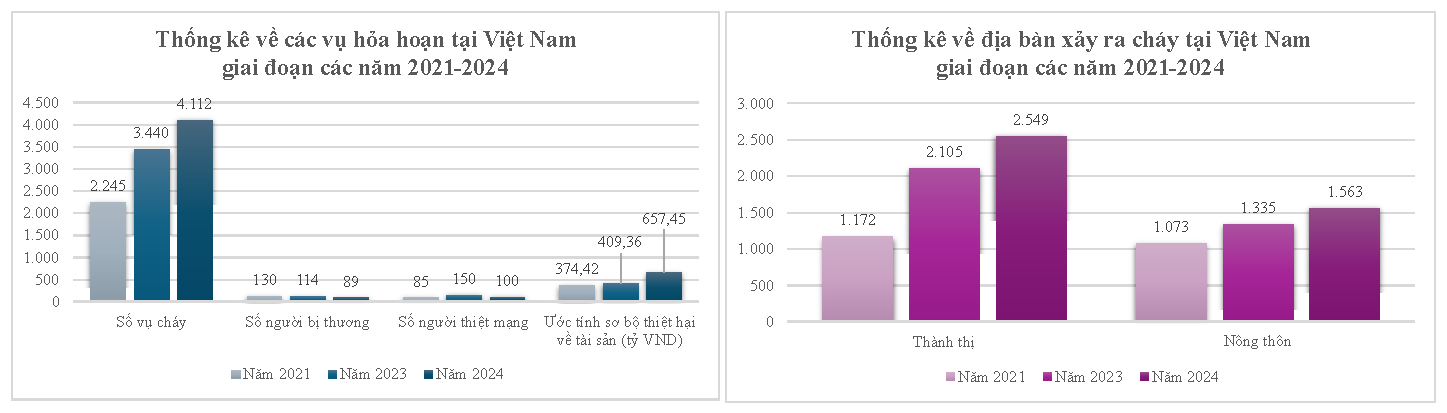
\includegraphics[width=0.85\linewidth]{Figure/tinh_hinh_chay_no.pdf}
    \caption{Thống kê tình hình cháy nổ qua các năm}
    \label{fig:tinh_hinh_chay}
\end{figure}

Lính cứu hỏa đóng vai trò then chốt trong các hoạt động ứng phó khẩn cấp và thường xuyên phải đối mặt với những nguy hiểm nghiêm trọng \cite{FirefighterImportant2022}. Các hiểm nguy phổ biến bao gồm nhiệt độ cực cao \cite{Firefighterhealthcare2024}, khí độc \cite{Firefighter_toxis}, không gian hẹp và nguy cơ sập đổ công trình. Theo thống kê của Hiệp hội Bảo vệ Phòng cháy Quốc gia Hoa Kỳ (NFPA), năm 2023 có 63.175 lính cứu hỏa bị thương với 89 trường hợp tử vong trong khi thi hành nhiệm vụ. Hoạt động dập tắt đám cháy chiếm tỉ lệ thương vong cao nhất, lên tới khoảng 18.875 trường hợp. Điều đáng chú ý là 87\% tổng số thương vong xảy ra trong các vụ cháy trong nhà, nơi xác suất thương tật vĩnh viễn cao gấp mười lần so với cháy ngoài nhà.

\begin{figure}[!htb]
    \centering
    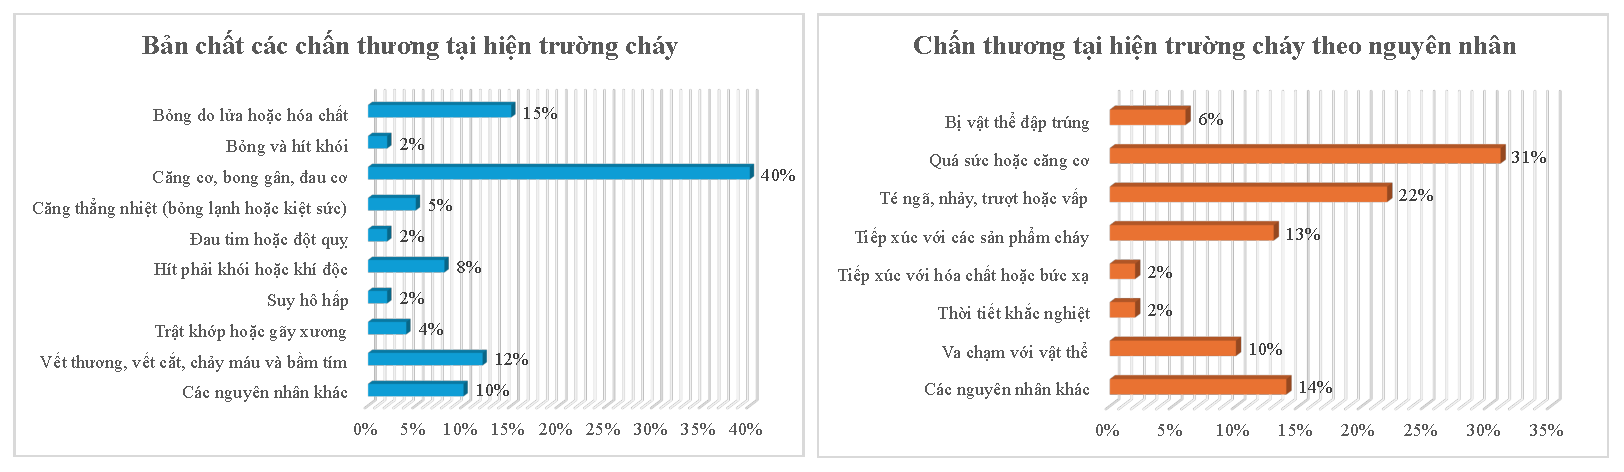
\includegraphics[width=0.85\linewidth]{Figure/nguyen_nhan_chan_thuong.pdf}
    \caption{Phân tích nguyên nhân chấn thương lính cứu hỏa}
    \label{fig:nguyen_nhan}
\end{figure}

Sự ứng dụng của khoa học công nghệ đã và đang nâng cao đáng kể mức độ an toàn của lính cứu hỏa \cite{FirefighterImportant2022, carmona2024firefighters}. Các hướng nghiên cứu chính hiện nay tập trung vào three lĩnh vực: (1) nâng cấp trang phục bảo hộ để giảm thiểu tác động của nhiệt và hóa chất \cite{FirefighterClothing2022}; (2) giám sát trạng thái tâm lý và sức khỏe trong điều kiện căng thẳng cao \cite{Firefighterhealthcare2024}; và (3) phát triển hệ thống giám sát hiện trường và liên lạc hỗ trợ ra quyết định \cite{Thanhfire2019, Firefighter_Falling_2023}.

\subsection{Tính cấp thiết của hệ thống giám sát hoạt động thời gian thực}

Việc giám sát liên tục hiệu suất hoạt động của lính cứu hỏa và duy trì liên lạc với trung tâm chỉ huy là yếu tố then chốt để phản ứng kịp thời và giảm thiểu rủi ro \cite{FirefighterImportant2022}. Tuy nhiên, các phương pháp liên lạc truyền thống như bộ đàm hai chiều chỉ cung cấp thông tin phân mảnh và thiếu khả năng theo dõi trạng thái theo thời gian thực của từng cá nhân \cite{Clifford2021}. Điều này gây cản trở đáng kể cho công tác phối hợp cứu hộ, đặc biệt khi không thể xác định vị trí hoặc trạng thái của một lính cứu hỏa do bất tỉnh hoặc bất động \cite{Zhang2024}.

Việc thiếu thông tin chính xác và liên tục về vị trí và trạng thái của từng lính cứu hỏa đặt ra những thách thức lớn cho công tác chỉ huy và phối hợp cứu hộ \cite{Firefighter_Falling_2023, Firefighterhealthcare2024}. Nhận dạng hoạt động lính cứu hỏa (FAR) kết hợp với thông tin vị trí là một hướng tiếp cận tiềm năng, cung cấp dữ liệu khách quan và liên tục, hỗ trợ ra quyết định kịp thời \cite{Accelerometerlocation2021}.

Khoảng trống nghiên cứu hiện tại thể hiện rõ ở ba điểm: (1) phần lớn nghiên cứu hiện có tập trung vào phát hiện ngã mà ít chú trọng đến nhận dạng toàn diện các hoạt động đặc thù của lính cứu hỏa như bò, trườn, đi khom; (2) thiếu tập dữ liệu công khai chuyên biệt cho lính cứu hỏa; (3) chưa có giải pháp tối ưu cho việc triển khai mô hình học máy trên vi điều khiển công suất thấp phù hợp với môi trường thi hành nhiệm vụ thực tế.

\subsection{Tổng quan nghiên cứu nhận dạng hoạt động con người}

\subsubsection{Phân loại phương pháp nhận dạng hoạt động}

Nhận dạng hoạt động con người được tiếp cận theo hai hướng chính: thị giác máy tính (computer vision) và tín hiệu cảm biến đeo (wearable sensor). Hướng thị giác máy tính gặp nhiều hạn chế trong môi trường chữa cháy thực tế do nhạy cảm với điều kiện ánh sáng và khói, yêu cầu xử lý dữ liệu phức tạp, đồng thời đặt ra lo ngại về quyền riêng tư \cite{HARvision2020}. Ngược lại, cảm biến đeo được đánh giá cao nhờ kích thước nhỏ gọn, chi phí thấp và khả năng phát hiện nhanh các thay đổi động học \cite{Accelerometer2021, DaoHieu2022, ViManhTuyen2024, HongNhung2023}.

\subsubsection{Học máy truyền thống trong nhận dạng hoạt động}

Học máy (ML) truyền thống được ứng dụng rộng rãi trong HAR nhờ tính đơn giản, phù hợp triển khai trên thiết bị đeo công suất thấp và khả năng cân bằng giữa chi phí, hiệu quả năng lượng và hiệu suất nhận dạng \cite{HongNhung2023, DaoHieu2022}. Thu và cộng sự \cite{Thu2022} đã triển khai cây quyết định (DT) để phân loại năm hoạt động cơ bản (nằm, ngồi, đứng, đi bộ, chạy bộ), đạt độ chính xác 99\% trên vi điều khiển ESP8266. Hong và cộng sự \cite{HongNhung2023} phát triển hệ thống tích hợp gia tốc kế, vi điều khiển công suất thấp và RF, đạt độ chính xác 99,2\% khi nhận dạng bốn trạng thái hoạt động cơ bản.

Lu và cộng sự \cite{Lu2020} đề xuất phương pháp HAR sử dụng một cảm biến gia tốc kế duy nhất, kết hợp đặc trưng toàn cục và cục bộ, đạt 93\% độ chính xác với các thuật toán GBDT, RF, KNN và SVM. Bên cạnh các đặc trưng miền thời gian, Preece và cộng sự \cite{preece2008_leutheuser2013_Lu2020} đã so sánh 14 loại đặc trưng từ tín hiệu gia tốc kế trên các miền thời gian, tần số và wavelet, xác nhận rằng đặc trưng miền tần số từ cảm biến đặt tại mắt cá chân cho phép phân loại tám hoạt động với độ chính xác tối đa 94\%.

\subsubsection{Học sâu trong nhận dạng hoạt động}

Học sâu (DL) thể hiện ưu thế vượt trội trong HAR nhờ khả năng tự động học đặc trưng từ tín hiệu cảm biến và mô hình hóa các mẫu hoạt động phức tạp \cite{DL2021_HAR_wearable}. Xu và cộng sự \cite{HAR_DCT_deeplearning2023} đề xuất cơ chế chú ý kênh dựa trên biến đổi cosine rời rạc (DCT) trong miền tần số, cải thiện hiệu suất mô hình ResNet lên 79,51\% trên UniMiB-SHAR. Qin và cộng sự \cite{HAR_CNN_2024} phát triển chiến lược học cộng tác với mô hình CLS-CNN-ResNest, đạt 99,12\% trên WISDM và hỗ trợ suy luận trực tiếp trên thiết bị thông qua cơ chế chia sẻ trọng số giữa các mạng con.

Tuy nhiên, học sâu thường đòi hỏi tài nguyên tính toán lớn, khiến chúng kém phù hợp với các thiết bị nhúng có tài nguyên hạn chế. Đối với các ứng dụng HAR thời gian thực, đặc biệt trên nền tảng vi điều khiển công suất thấp, ML truyền thống vẫn là lựa chọn thực tế hơn nhờ tính đơn giản, chi phí thấp và khả năng triển khai hiệu quả.

\begin{table}[!htb]
    \centering
    \caption{Tổng quan các nghiên cứu HAR sử dụng thiết bị đeo}
    \label{tab:har_overview}
    \footnotesize
    \renewcommand{\arraystretch}{1.2}
    \resizebox{\linewidth}{!}{
    \begin{tabular}{
        >{\centering\arraybackslash}m{0.08\linewidth}
        >{\RaggedRight\arraybackslash}m{0.52\linewidth}
        >{\RaggedRight\arraybackslash}m{0.12\linewidth}
        >{\RaggedRight\arraybackslash}m{0.22\linewidth}
    }
        \hline\hline
        \rowcolor{gray!20}\textbf{Năm} & \textbf{Tập dữ liệu} & \textbf{Đối tượng} & \textbf{Phương pháp} \\
        \hline\hline
        2024 & Accelerometer; UniMiB (50~Hz), WISDM (20~Hz), UCI (50~Hz); túi trước & Người, HĐ & CLS-CNN-ResNest \cite{HAR_CNN_2024}\\
        \hline
        2024 & Fusion sensors; 100~Hz; 18 TV; cánh tay, bắp tay, bắp chân; 8 HĐ & Lính CỐH, HĐ & Hybrid ML \cite{CHAI_FIRE2024}\\
        \hline
        2023 & Accelerometer; UniMiB (50~Hz), UR Fall (256~Hz), UCI (50~Hz) & Người, HĐ & CNN-DCT \cite{HAR_DCT_deeplearning2023}\\
        \hline
        2022 & Accelerometer, CO; 100~Hz; 8 TV; thắt lưng; 2 HĐ & Lính CỐH, ngã & Fall detection \cite{Dang2022}\\
        \hline
        2021 & 9-axis, 15~Hz; 10 TV; ngực, khuỷu, thắt lưng, đùi, mắt cá; 2 HĐ & Lính CỐH, ngã & LSTM \cite{Chai2021}\\
        \hline
        2020 & Accelerometer; 50~Hz; 21 TV; cổ tay; 6 HĐ & Người, HĐ & GBDT, RF, KNN, SVM \cite{Lu2020}\\
        \hline
        2019 & 9-axis, CO; barometer; 100~Hz; 6 TV; túi quần; 2 HĐ & Lính CỐH, ngã & Fall detection \cite{Thanhfire2019}\\
        \hline
        2016 & RF, doppler; 20~Hz; ngực, trán, cổ tay phải, mắt cá phải; 7 HĐ & Lính CỐH, HĐ & SVM \cite{Geng2016}\\
        \hline\hline
    \end{tabular}}
    \footnotesize \textit{Chú thích: TV = tình nguyện viên; HĐ = hoạt động; Lính CỐH = Lính cứu hỏa}
\end{table}

\subsection{Tổng quan nghiên cứu nhận dạng hoạt động lính cứu hỏa}

Hệ thống nhận dạng hoạt động lính cứu hỏa (FAR) phải xử lý các chuyển động động và cường độ cao trong môi trường nguy hiểm. Mục tiêu của các hệ thống này là nâng cao an toàn và hiệu quả hoạt động bằng cách giám sát thể chất, phát hiện bất thường và cung cấp thông tin thời gian thực trong tình huống khẩn cấp \cite{Firefighterhealthcare2024, Thanhfire2019}.

Geng và cộng sự \cite{Geng2016} giới thiệu phương pháp nhận dạng hoạt động lính cứu hỏa dựa trên tín hiệu tần số vô tuyến, sử dụng SVM với nhân Gaussian để phân biệt bảy hoạt động. Hệ thống đạt độ chính xác trung bình 88,7\%, trong đó các hoạt động tĩnh như đứng và nằm được nhận dạng chính xác hơn. Tuy nhiên, cửa sổ thời gian 10 giây hạn chế khả năng phản hồi nhanh với các hoạt động phức tạp và nhanh của lính cứu hỏa.

Pham và cộng sự \cite{Thanhfire2019} phát triển hệ thống hỗ trợ kết hợp thuật toán cảm biến hợp nhất để phát hiện ngã, giám sát tình trạng thể chất và đánh giá điều kiện môi trường. Thuật toán phát hiện ngã kết hợp dữ liệu gia tốc, tư thế và độ cao, đạt 100\% độ chính xác trên tập dữ liệu thực nghiệm riêng và 97,9\% trên tập dữ liệu công khai. Dang và cộng sự \cite{Dang2022} phát triển hệ thống hỗ trợ thời gian thực sử dụng gia tốc kế và cảm biến CO, đạt độ chính xác phát hiện ngã 93\% với độ nhạy 96,5\%. Chai và cộng sự \cite{Chai2021} phát triển hệ thống phát hiện ngã thông minh, tích hợp cảm biến vào trang phục bảo hộ tại năm vị trí cơ thể và sử dụng mạng LSTM ba lớp, đạt độ chính xác 94,1\%.

Nhìn chung, các nghiên cứu hiện tại chủ yếu tập trung vào phát hiện ngã mà chưa nhận dạng toàn diện các hoạt động đặc thù như bò (CR), trườn (SL), đi khom (WS). Hơn nữa, phần lớn nghiên cứu chưa giải quyết vấn đề nhận dạng chuyển tiếp giữa các hoạt động trong kịch bản thời gian thực, cũng như chưa tối ưu hóa cho triển khai trên vi điều khiển công suất thấp.

\subsection{TinyML và triển khai mô hình trên thiết bị biên}

TinyML là lĩnh vực nghiên cứu tập trung vào việc chạy suy luận học máy trực tiếp trên các thiết bị biên có tài nguyên hạn chế — thường có bộ nhớ Flash dưới 1~MB và RAM vài trăm KB \cite{SurveyTinyML2023}. Cách tiếp cận này mang lại lợi thế đáng kể về độ trễ thấp, tiết kiệm băng thông, tăng cường quyền riêng tư dữ liệu và khả năng hoạt động ngoại tuyến.

Saha và cộng sự \cite{MLforMicrocontroller2022} đã tổng quan các phương pháp học máy cho phần cứng cấp vi điều khiển, xác nhận rằng RF và các biến thể cây quyết định là nhóm thuật toán phù hợp nhất cho triển khai trên MCU điện năng thấp. Nghiên cứu của Vi và cộng sự \cite{ViManhTuyen2024} và Dao và cộng sự \cite{DaoHieu2022} đã chứng minh tính khả thi của việc triển khai RF trực tiếp trên vi điều khiển ESP32 và các MCU hiệu suất thấp tương tự, đạt hiệu suất nhận dạng cao với độ trễ chấp nhận được trong ứng dụng HAR thực tế.

Thư viện micromlgen cho phép chuyển đổi mô hình scikit-learn đã huấn luyện sang mã C/C++ tương thích với Arduino và ESP32, tạo điều kiện để tích hợp trực tiếp vào firmware thiết bị nhúng \cite{Tiny_machine_on_microcontroller}. Các nghiên cứu gần đây \cite{TinyMLOnEmbedded2025, RIOT_tinyML2025} xác nhận rằng các mô hình TinyML có thể hoạt động ổn định trong điều kiện tài nguyên hạn chế, với kích thước triển khai điển hình trong khoảng 0,5--1,0~MB flash.

\subsection{Mục tiêu, phạm vi và đóng góp của đề tài}

Dựa trên những khoảng trống nghiên cứu đã xác định, đề tài đặt ra mục tiêu xây dựng hệ thống RFAR --- hệ thống nhận dạng hoạt động lính cứu hỏa theo thời gian thực --- có khả năng phân loại chính xác mười một hoạt động đặc thù của lính cứu hỏa trong môi trường cứu hộ khẩn cấp, triển khai trên thiết bị đeo nhỏ gọn sử dụng vi điều khiển công suất thấp.

Đề tài hướng tới bốn đóng góp chính:

\begin{enumerate}[leftmargin=1.5cm, label=(\arabic*)]
    \item \textbf{Tập dữ liệu chuyên biệt:} Xây dựng tập dữ liệu mô phỏng các hoạt động lính cứu hỏa trong buổi diễn tập cứu nạn, bổ sung khoảng trống trong các tập dữ liệu công khai hiện có.
    \item \textbf{Quy trình xử lý tín hiệu mới:} Đề xuất pipeline kết hợp kỹ thuật cửa sổ trượt với phát hiện chỉ số bất thường (AIx) để cải thiện chất lượng thông tin hoạt động và xử lý hiệu quả các chuyển tiếp giữa hoạt động.
    \item \textbf{Hệ thống RFAR tối ưu:} Phát triển hệ thống sử dụng thiết bị đeo gia tốc kế tại thắt lưng để nhận dạng mười một hoạt động, triển khai mô hình RF tối ưu trên vi điều khiển công suất thấp với kích thước dưới 1~MB.
    \item \textbf{Thiết bị đeo thực tế:} Chế tạo thiết bị đeo có trọng lượng dưới 200~g, khả năng hoạt động liên tục 24~giờ, được xác nhận trong thực nghiệm thực tế với điểm F1$>$96\%.
\end{enumerate}

Về phạm vi của báo cáo tiến độ này, nghiên cứu đã hoàn thành các mục tiêu cốt lõi của giai đoạn hiện tại bao gồm xây dựng tập dữ liệu, phát triển và tối ưu hóa hệ thống, cùng thực nghiệm xác nhận. Các hướng mở rộng như tích hợp định vị trong nhà và mạng lưới giám sát tập trung đang được lên kế hoạch cho các giai đoạn tiếp theo.


\pagebreak

\section{VẬT LIỆU VÀ PHƯƠNG PHÁP}
\label{materials_and_methods}

\subsection{Kiến trúc hệ thống RFAR đề xuất}

\subsubsection{Tổng quan hệ thống}

Hình~\ref{fig:system} minh họa kiến trúc tổng thể và luồng hoạt động của hệ thống RFAR đề xuất. Hệ thống được thiết kế nhằm hỗ trợ trung tâm chỉ huy theo dõi trạng thái hoạt động của từng thành viên đội cứu hộ theo thời gian thực. Mỗi lính cứu hỏa được trang bị một thiết bị đeo nhỏ gọn gắn tại vùng thắt lưng, có khả năng nhận dạng và truyền dữ liệu hoạt động thời gian thực đến thiết bị trung tâm do chỉ huy kiểm soát. Thiết bị trung tâm hiển thị trực quan trạng thái hoạt động của các thành viên, hỗ trợ ra quyết định kịp thời trong tình huống khẩn cấp.

\begin{figure}[!htb]
    \centering
    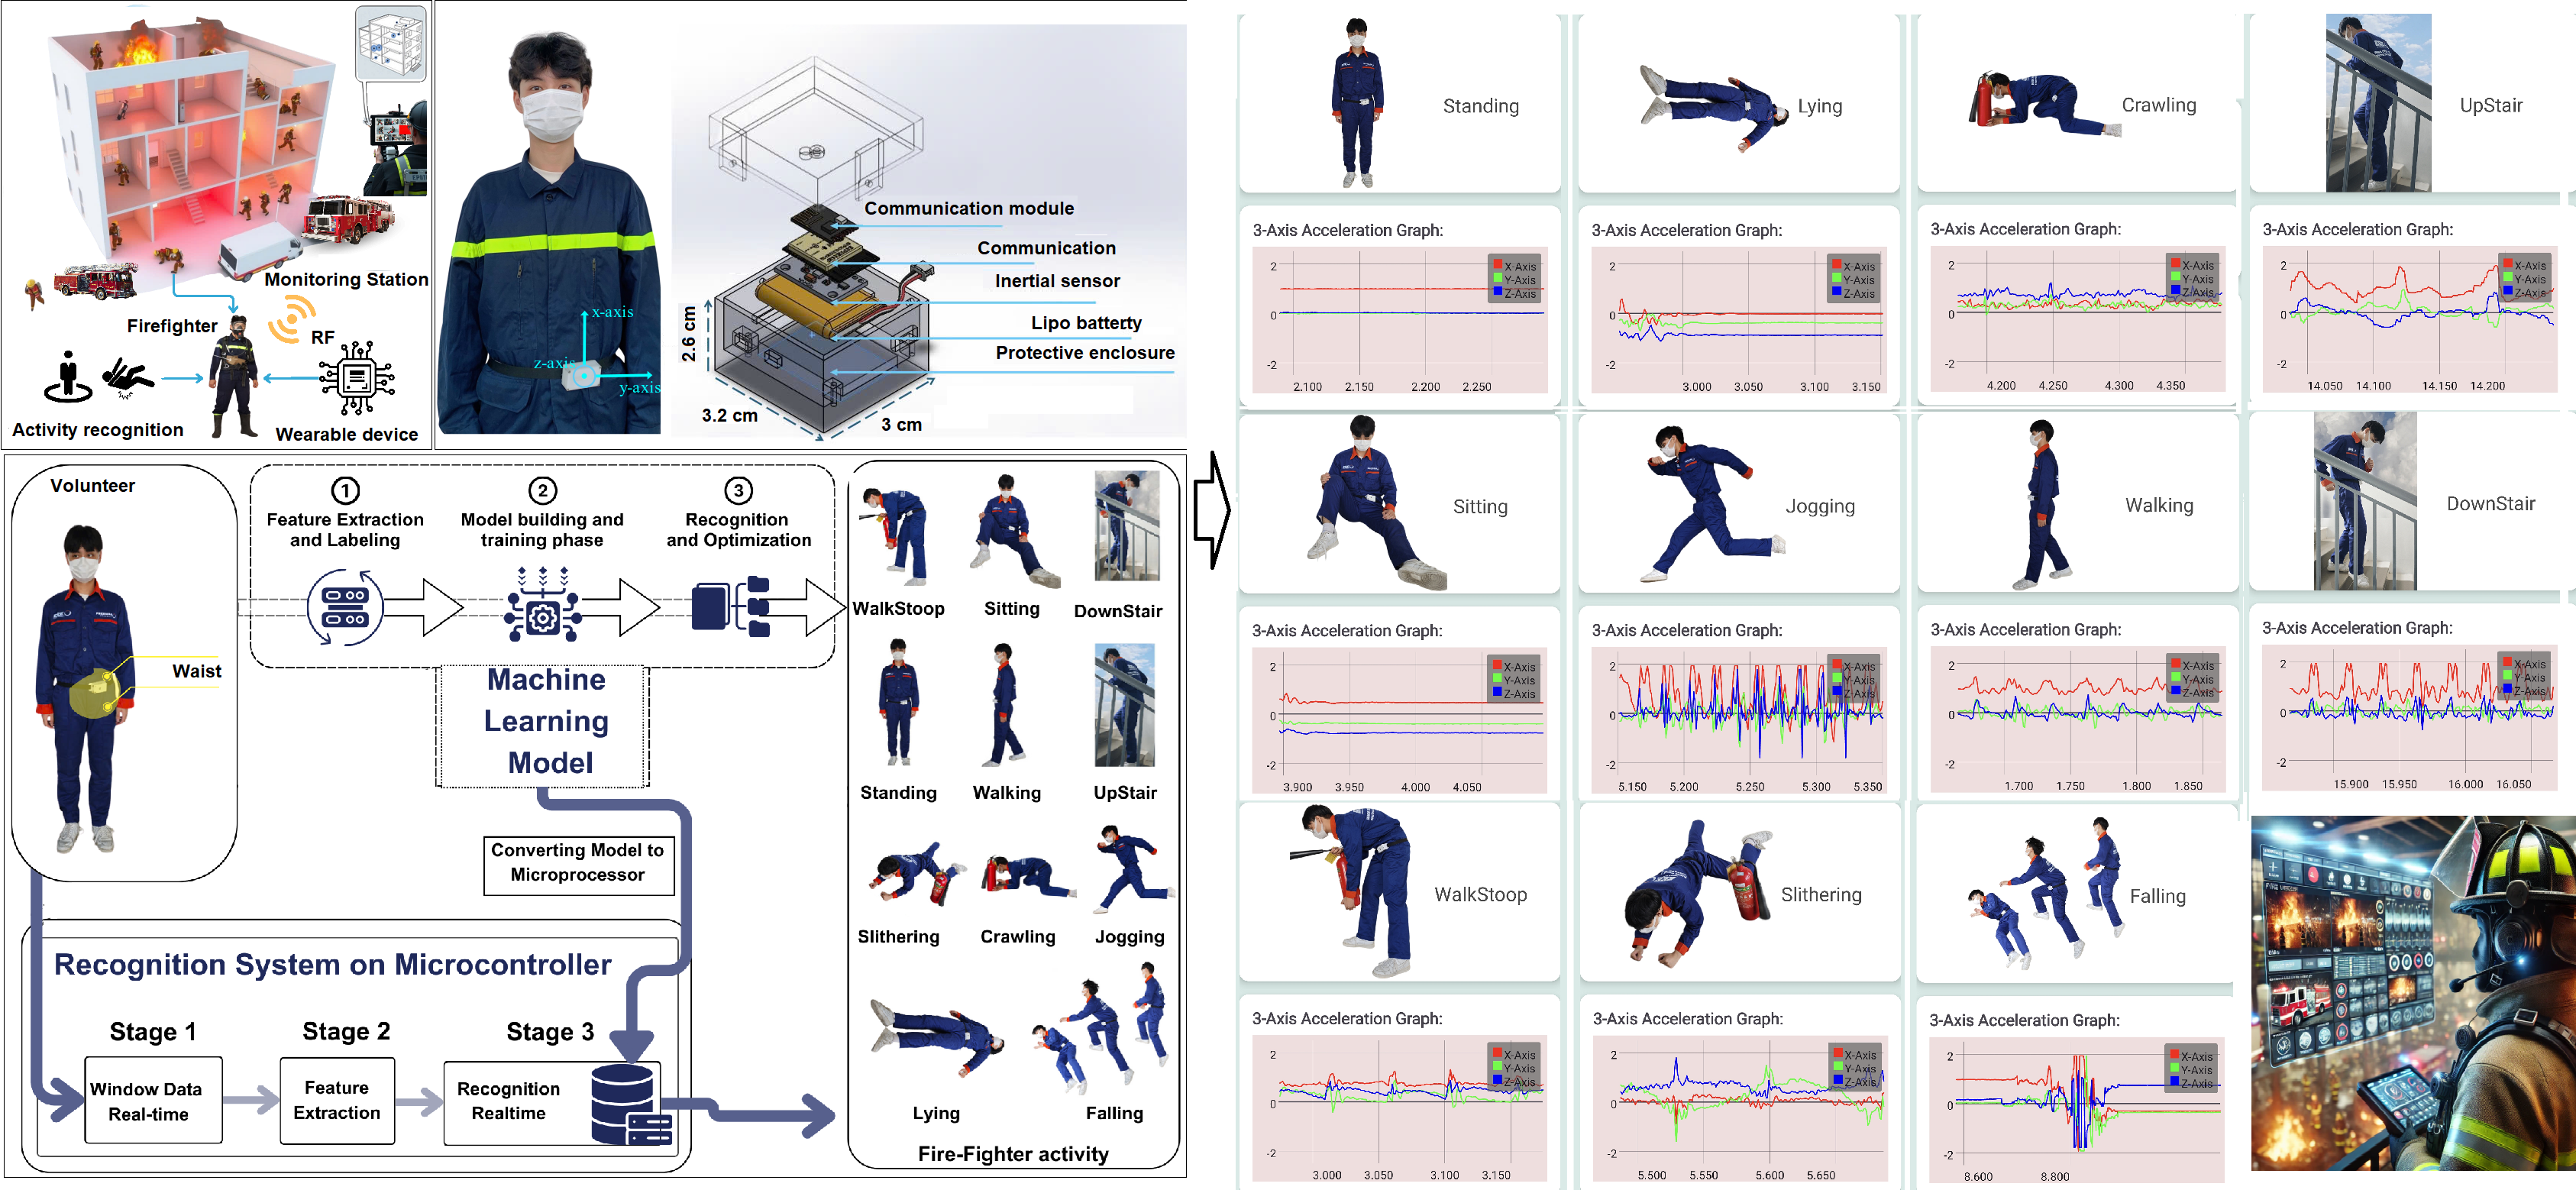
\includegraphics[width=1\linewidth]{Figure/FirefighterSystemfull.png}
    \caption{Kiến trúc tổng thể hệ thống RFAR nhận dạng hoạt động lính cứu hỏa thông qua thiết bị đeo tại thắt lưng, giao tiếp với màn hình chỉ huy qua sóng vô tuyến}
    \label{fig:system}
\end{figure}

\subsubsection{Cấu hình phần cứng}

Cấu hình chi tiết của hệ thống được trình bày trong Bảng~\ref{tab:hardware}. Thiết bị đeo bao gồm cảm biến gia tốc kế ADXL345 ba trục và vi điều khiển ESP32 với 520~KB RAM, 448~KB ROM và 4~MB Flash. Module truyền thông hoạt động ở tần số 433~MHz, đảm bảo khoảng cách truyền tải lên đến 8000~m với tốc độ 2,4~Kbps. Nguồn điện được cung cấp bởi pin Li-ion 2000~mAh, đảm bảo khả năng hoạt động liên tục trên 24~giờ. Toàn bộ thiết bị có trọng lượng dưới 200~g, phù hợp để gắn lên trang phục bảo hộ của lính cứu hỏa.

\begin{table}[!htb]
    \caption{Cấu hình phần cứng và nền tảng thực nghiệm}
    \label{tab:hardware}
    \centering
    \footnotesize
    \renewcommand{\arraystretch}{1.2}
    \resizebox{\linewidth}{!}{
    \begin{tabular}{
        >{\centering\arraybackslash}m{0.15\linewidth}
        >{\arraybackslash}m{0.22\linewidth}
        >{\arraybackslash}m{0.58\linewidth}}
    \hline\hline
    \rowcolor{gray!20}\textbf{Module} & \textbf{Linh kiện} & \textbf{Thông số kỹ thuật} \\
    \hline\hline
    \multirow{5}{*}{\makecell{Thiết bị\\đeo}} & ADXL345 & Gia tốc kế 3 trục kỹ thuật số \\
    & ESP32 & 520~KB RAM, 448~KB ROM, 4~MB Flash \\
    & Thẻ Micro SD & 2~GB \\
    & Truyền thông & 433~MHz; 8000~m; 2,4~Kbps \\
    & Pin & Li-ion, 2000~mAh \\
    \hline
    \multirow{3}{*}{\makecell{Thiết bị\\trung tâm}} & Truyền thông & 433~MHz; 8000~m; 2,4~Kbps \\
    & ESP32 & 520~KB RAM, 448~KB ROM, 4~MB Flash \\
    & Nguồn điện & Bộ chuyển đổi 12~VDC--2A \\
    \hline
    \multirow{5}{*}{Máy chủ} & Chipset & Intel Xeon Silver 4310; 2,1~GHz \\
    & RAM & 16~GB RDIMM \\
    & Ổ cứng & 2~TB IDD NLSAS \\
    & Phần mềm & Visual Studio Code \\
    & Giao thức & MQTT \\
    \hline\hline
    \end{tabular}}
\end{table}

Hệ thống có khả năng nhận dạng mười một hoạt động bao gồm: đi bộ (WA), đứng (ST), nằm (LY), ngồi (SI), chạy bộ (JO), đi khom (WS), bò tay-gối (CR), trườn sát đất (SL), ngã (FA), xuống cầu thang (DS) và lên cầu thang (US). Hệ thống hoạt động theo ba giai đoạn tuần tự: thu thập dữ liệu thời gian thực qua cửa sổ trượt, trích xuất đặc trưng và nhận dạng hoạt động.

\subsection{Xây dựng cơ sở dữ liệu}

\subsubsection{Tập dữ liệu riêng}

Tập dữ liệu lính cứu hỏa được thu thập từ nhóm 20 tình nguyện viên nam trong tình trạng sức khỏe tốt, có độ tuổi từ 22 đến 35, chiều cao từ 1,6 đến 1,8~m và cân nặng từ 60 đến 80~kg. Các tình nguyện viên được tuyển chọn từ Trường Đại học Phenikaa và Trường Đại học Phòng cháy Chữa cháy, không có tình nguyện viên nữ tham gia nhằm đảm bảo đồng nhất về đặc điểm thể chất phù hợp với đối tượng nghiên cứu là lính cứu hỏa nam. Dữ liệu được thu thập tại tần số lấy mẫu 100~Hz, ghi lại giá trị gia tốc ba trục theo đơn vị $g$ ($g = 9{,}8$~m/s$^2$), trong quá trình diễn tập cứu nạn thực tế.

\begin{table}[!htb]
    \caption{Mô tả các hoạt động lính cứu hỏa trong tập dữ liệu riêng}
    \label{tab:activity}
    \centering
    \footnotesize
    \renewcommand{\arraystretch}{1.2}
    \resizebox{\linewidth}{!}{
    \begin{tabular}{>{\centering\arraybackslash}m{0.08\linewidth}m{0.70\linewidth}m{0.12\linewidth}}
    \hline\hline
    \rowcolor{gray!20}\textbf{HĐ} & \textbf{Mô tả} & \textbf{Mẫu} \\
    \hline\hline
    WA & Di chuyển thẳng đứng, duy trì ít nhất một bàn chân tiếp xúc mặt đất & 123.932 \\
    \hline
    ST & Duy trì tư thế thẳng đứng không di chuyển & 56.016 \\
    \hline
    LY & Đặt cơ thể trên mặt phẳng, lưng tiếp xúc mặt đất & 82.516 \\
    \hline
    SI & Tư thế nghỉ với mông và bàn chân tiếp xúc mặt đất & 63.013 \\
    \hline
    JO & Trạng thái di chuyển nhanh, không quá một bàn chân tiếp xúc mặt đất cùng lúc & 90.783 \\
    \hline
    WS & Đi bộ chậm trong tư thế gập hoặc khom lưng & 83.242 \\
    \hline
    CR & Di chuyển về phía trước bằng tay và gối, thân trên nâng nhẹ khỏi mặt đất & 82.669 \\
    \hline
    SL & Di chuyển sát đất bằng tay và gối, cơ thể song song với mặt đất & 90.340 \\
    \hline
    FA & Mất thăng bằng đột ngột dẫn đến tiếp xúc với mặt đất & 129.815 \\
    \hline
    DS & Xuống cầu thang bằng bộ với tốc độ vừa phải & 151.448 \\
    \hline
    US & Lên cầu thang bằng bộ với tốc độ vừa phải & 157.882 \\
    \hline\hline
    \end{tabular}}
    \footnotesize \textit{Chú thích: HĐ = Hoạt động}
\end{table}

Bảng~\ref{tab:activity} trình bày mô tả chi tiết và số lượng mẫu của từng hoạt động. Mỗi hoạt động được thực hiện liên tục ít nhất ba phút, ngoại trừ hoạt động ngã (FA) được thực hiện trong khoảng 3--5 giây. Dữ liệu được lưu trữ trên thẻ nhớ microSD gắn tại thiết bị đeo ở vùng thắt lưng. Tổng thời gian thu thập dữ liệu là 371~phút với tổng kích thước dữ liệu vượt quá 100~MB. Tập dữ liệu được phân chia theo tỉ lệ 60/40 cho tập huấn luyện và kiểm tra.

\subsubsection{Các tập dữ liệu công khai}

Để đánh giá tính khái quát của phương pháp, nghiên cứu sử dụng thêm ba tập dữ liệu công khai có chứa các hoạt động tương đồng:

\begin{itemize}
    \item \textbf{MobiFall} \cite{MobiFall2015}: Bao gồm bốn loại ngã và chín hoạt động sinh hoạt hàng ngày, được thu thập bằng điện thoại thông minh đặt trong túi.
    \item \textbf{SFDLA} \cite{SFDLAdataset2016}: Tập dữ liệu phát hiện ngã và hoạt động dựa trên cảm biến đặt cố định tại thắt lưng.
    \item \textbf{UniMiB-SHAR} \cite{UniMiB_SHAR_2017}: Bao gồm 17 hoạt động từ điện thoại thông minh đặt trong túi trước với hướng cảm biến thay đổi giữa các phiên.
\end{itemize}

Nghiên cứu này áp dụng cách tiếp cận mới, coi ngã là một hành vi cần nhận dạng thay vì coi đó là sự kiện tách biệt, tạo cơ sở so sánh khách quan với các nghiên cứu trước đây về phát hiện ngã và nhận dạng hoạt động.

\subsection{Quy trình xử lý dữ liệu}

\subsubsection{Giảm tần số lấy mẫu}

Để tối ưu hiệu quả xử lý, tần số lấy mẫu được giảm từ 100~Hz xuống 50~Hz thông qua bộ lọc trung bình trượt. Với mỗi trục $k \in \{x, y, z\}$, tín hiệu sau giảm mẫu $a_k[n]$ được tính theo công thức:

\begin{equation}
a_k[n] = \frac{\bar{a}_k[2n - 1] + \bar{a}_k[2n]}{2}, \quad n \in [1, N]
\label{eq:resample}
\end{equation}

trong đó $\bar{a}_k$ là tín hiệu gốc tại 100~Hz, $N = \bar{N}/2$ là độ dài tín hiệu sau giảm mẫu, và $F_s = 50$~Hz là tần số lấy mẫu kết quả. Việc giảm mẫu này giảm đáng kể yêu cầu tính toán và tiêu thụ năng lượng trong khi thực nghiệm cho thấy chỉ cải thiện không đáng kể (0,2--0,3\%) khi tăng lên 100~Hz.

\subsubsection{Phân đoạn tín hiệu bằng cửa sổ trượt}

Tín hiệu liên tục $s[n]$ được phân đoạn thành các cửa sổ thời gian cố định với $\Delta t = 3$~giây (150 mẫu tại 50~Hz). Mỗi cửa sổ $W_j[n]$ chứa $M$ mẫu của ba thành phần gia tốc:

\begin{equation}
W_j[n] = (a_x[n], a_y[n], a_z[n]), \quad n \in [n_i, n_{i+1}], \quad j \in [1, N_{\Delta t}]
\end{equation}

Thực nghiệm cho thấy cửa sổ 3 giây là sự cân bằng thực tế: điểm F1 chỉ thấp hơn khoảng 2--3\% so với cửa sổ 6 giây, nhưng giảm đáng kể vấn đề chồng lấp hoạt động và giảm yêu cầu tài nguyên so với các cửa sổ dài hơn.

\subsubsection{Pipeline phát hiện ngã mới}

Hình~\ref{fig:pipeline} minh họa pipeline xử lý dữ liệu mới được đề xuất, trong đó phần nổi bật (màu xanh đậm) biểu thị quy trình mới so với phương pháp cửa sổ trượt thông thường (mũi tên xanh lá). Điểm khác biệt then chốt là thay vì sử dụng cửa sổ trượt cố định cho tất cả hoạt động, hệ thống tạo ra một cửa sổ dữ liệu chuyên biệt bao quanh vùng bất thường khi phát hiện sự kiện ngã.

\begin{figure}[!htb]
    \centering
    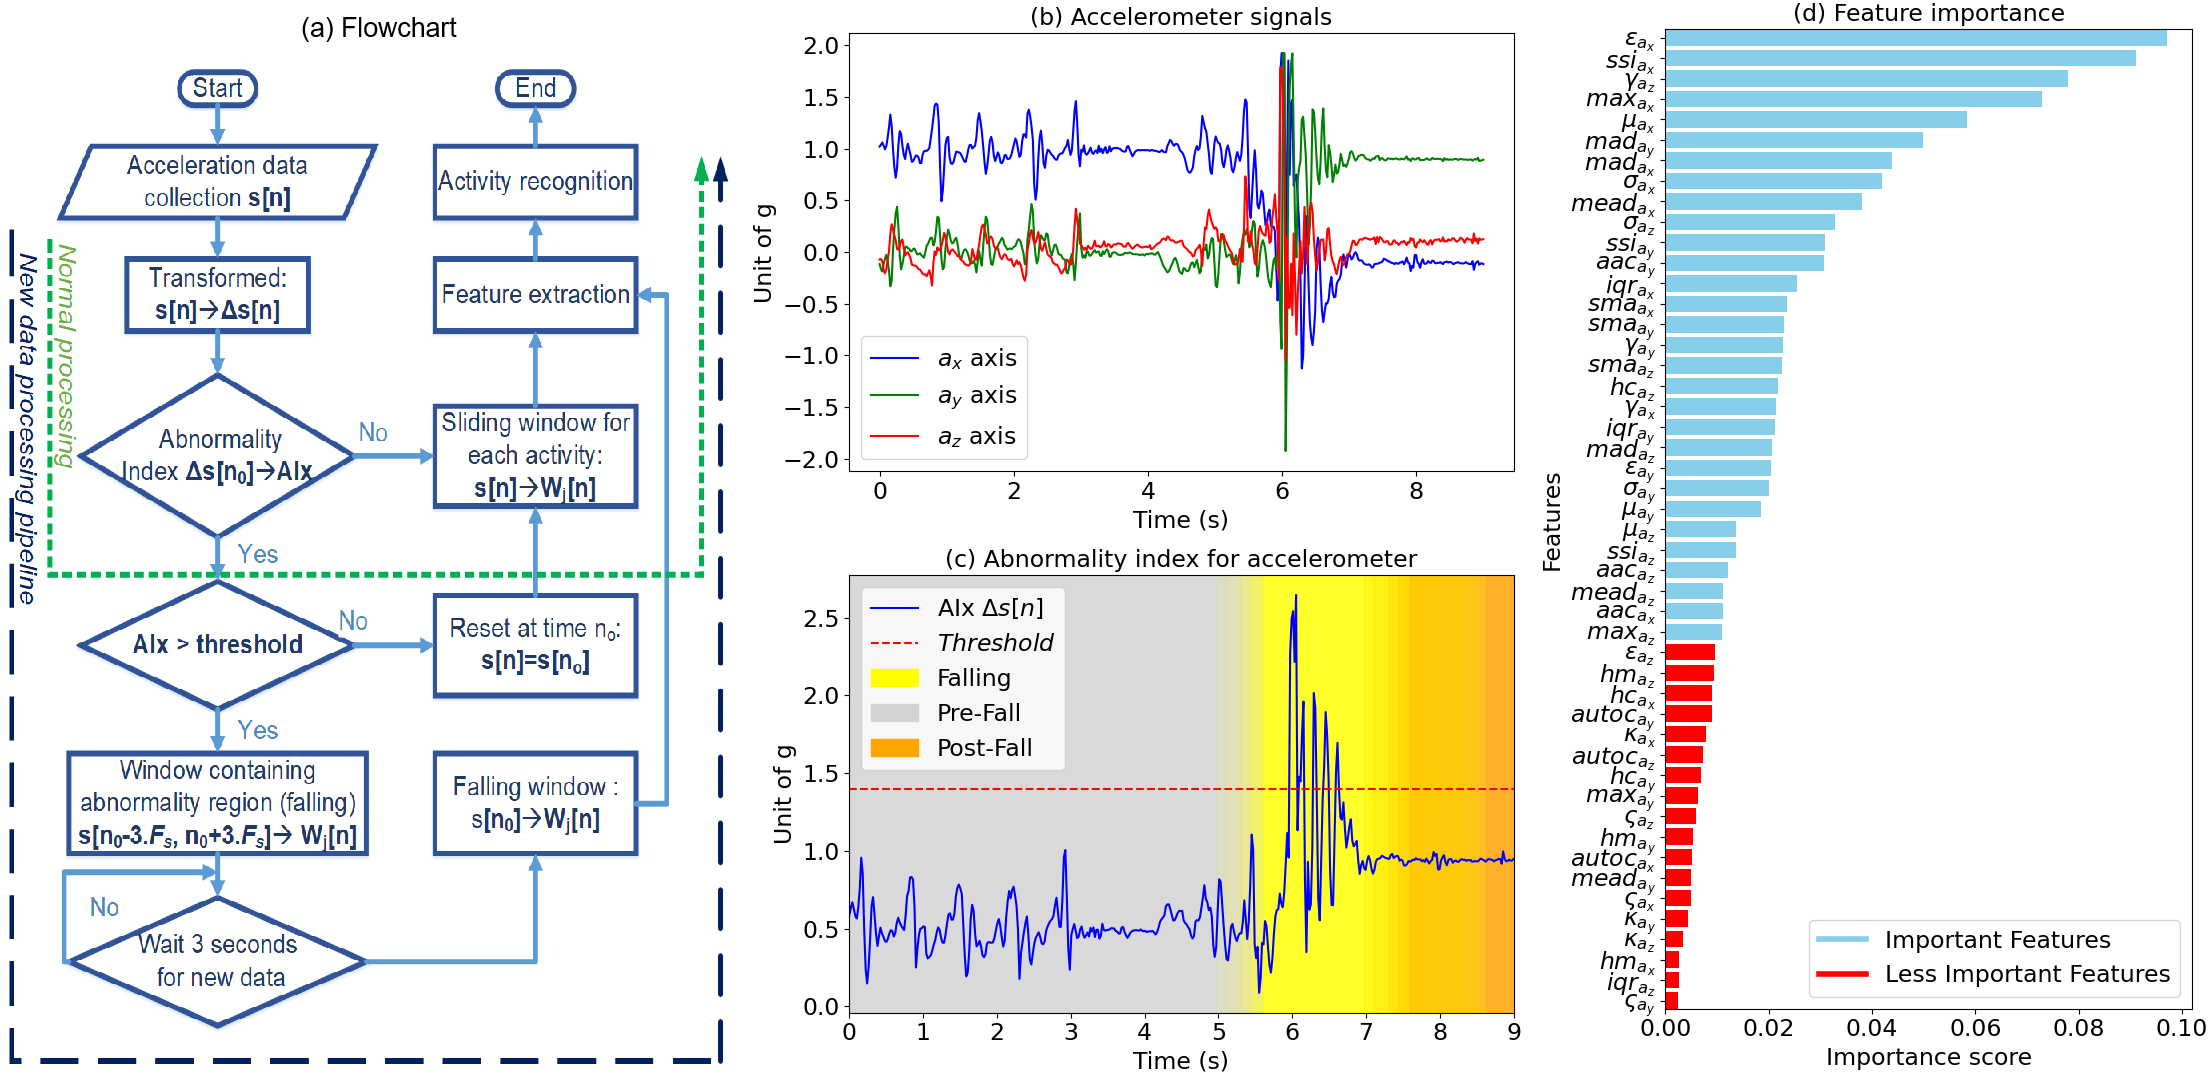
\includegraphics[width=1\linewidth]{Figure/pipeline.png}
    \caption{Sơ đồ pipeline phát hiện bất thường và xử lý dữ liệu: (a) lưu đồ pipeline tổng thể, (b) biến thiên tín hiệu trong hoạt động ngã, (c) kết quả phát hiện bất thường, (d) mức độ quan trọng đặc trưng}
    \label{fig:pipeline}
\end{figure}

\paragraph{Bước 1: Phát hiện chỉ số bất thường}

Chỉ số bất thường ($AIx$) biểu thị sự biến đổi đột ngột trong tín hiệu gia tốc kế tại một thời điểm cụ thể. $AIx$ được tính bằng cách biến đổi tín hiệu $s[n]$ thành chuỗi biến thiên $\Delta s[n]$:

\begin{equation}
\Delta s[n] = \sqrt{\sum_{k \in \{x, y, z\}} \left( a_k[n] - \frac{1}{N} \sum_{n=1}^{N} a_k[n] \right)^2}
\label{eq:delta_s}
\end{equation}

Chỉ số bất thường được xác định khi $\Delta s[n_0]$ vượt ngưỡng $threshold = 1{,}8g$:

\begin{equation}
AIx = \begin{cases}
\Delta s[n_0], & \text{nếu } \Delta s[n_0] > threshold = 1{,}8\,g \\
0, & \text{ngược lại}
\end{cases}
\label{eq:AIx}
\end{equation}

Ngưỡng cửa sổ phát hiện nhỏ $\Delta W = 0{,}5$~giây được chọn dựa trên thời gian tối thiểu của giai đoạn bay trong sự kiện ngã (khoảng 0,34~giây) \cite{Elder_Falling_2019}.

\paragraph{Bước 2: Thu thập dữ liệu xung quanh sự kiện bất thường}

Sau khi phát hiện bất thường tại thời điểm $n_0$, hệ thống thu thập thêm dữ liệu trong vùng:

\begin{equation}
W_j[n], \quad n \in [n_0 - 3 \cdot F_s, \; n_0 + 3 \cdot F_s]
\end{equation}

Cách tiếp cận này tạo ra một cửa sổ dữ liệu chuyên biệt 6 giây xung quanh điểm ngã, tập trung vào vùng tín hiệu quan trọng và cải thiện hiệu suất phát hiện so với cửa sổ trượt cố định.

\paragraph{Bước 3: Phân tích và phân loại}

Dữ liệu trong cửa sổ chuyên biệt này được phân tích để xác định mức độ nghiêm trọng của sự kiện ngã thông qua trích xuất đặc trưng và phân loại. Trong điều kiện bình thường, bước nhảy cửa sổ được đặt bằng kích thước cửa sổ (3~giây) để tiết kiệm năng lượng. Khi $AIx$ vượt ngưỡng, bước nhảy giảm xuống 0,5~giây để tăng tần suất nhận dạng.

\subsubsection{Gán nhãn dữ liệu}

Quy trình gán nhãn gồm ba bước: (1) xác định 11 nhãn tương ứng 11 hoạt động (0 đến 10); (2) phân đoạn và gán nhãn tuần tự theo từng hoạt động; (3) gán nhãn $L_j = k$ cho mỗi cửa sổ $W_j[n]$ thuộc hoạt động $k$. Tất cả hoạt động được quan sát và gán nhãn thủ công bởi hai người giám sát để đảm bảo tính chính xác của dữ liệu.

\subsection{Trích xuất đặc trưng}

\subsubsection{Lựa chọn đặc trưng miền thời gian}

Nghiên cứu ưu tiên các đặc trưng miền thời gian do phù hợp với yêu cầu triển khai trên MCU: không cần biến đổi Fourier tốn kém và có độ phức tạp tính toán thấp. Từ 16 loại đặc trưng ban đầu được xem xét, phương pháp loại trừ dựa trên mức độ quan trọng được áp dụng: giữ lại các đặc trưng có mức độ quan trọng lớn hơn hoặc bằng ngưỡng $0{,}01$ (bằng một nửa độ lệch chuẩn của phân phối mức độ quan trọng, xem Hình~\ref{fig:pipeline}-d).

\subsubsection{Tập đặc trưng tối ưu}

Kết quả lựa chọn cho ra 30 giá trị đặc trưng từ 13 loại đặc trưng. Bảng~\ref{tab:feature} tóm tắt thông tin mô tả các đặc trưng được sử dụng.

\begin{table}[!htb]
    \caption{Các đặc trưng tối ưu được sử dụng trong hệ thống}
    \label{tab:feature}
    \centering
    \footnotesize
    \renewcommand{\arraystretch}{1.5}
    \resizebox{\linewidth}{!}{
    \begin{tabular}{m{0.20\linewidth}m{0.06\linewidth}m{0.38\linewidth}m{0.32\linewidth}}
    \hline\hline
    \rowcolor{gray!20}\textbf{Loại đặc trưng} & \textbf{Trục} & \textbf{Mô tả} & \textbf{Công thức} \\
    \hline\hline
    Năng lượng & x, y & Căn bậc hai của trung bình bình phương tín hiệu &
    $\varepsilon_{a_k} = \sqrt{\frac{1}{M}\sum_{n=1}^{M}a_k^2[n]}$ \\
    Độ lệch tuyệt đối trung bình & x, y, z & Trung bình lệch so với giá trị trung bình &
    $\text{mad}_{a_k} = \frac{1}{M}\sum_{n=1}^{M}|a_k[n]-\mu_{a_k}|$ \\
    Diện tích độ lớn tín hiệu & x, y, z & Tổng giá trị tuyệt đối &
    $\text{sma}_{a_k} = \sum_{n=1}^{M}|a_k[n]|$ \\
    Trung bình & x, y, z & Giá trị trung bình tín hiệu &
    $\mu_{a_k} = \frac{1}{M}\sum_{n=1}^{M}a_k[n]$ \\
    Độ lệch chuẩn & x, y, z & Phân tán tín hiệu quanh giá trị trung bình &
    $\sigma_{a_k} = \sqrt{\frac{1}{M}\sum_{n=1}^{M}(a_k[n]-\mu_{a_k})^2}$ \\
    Tích phân bình phương đơn giản & x, y, z & Tổng bình phương các mẫu &
    $\text{ssi}_{a_k} = \sum_{n=1}^{M}a_k^2[n]$ \\
    Biến đổi biên độ trung bình & x, y, z & Trung bình biến thiên giữa các mẫu liền kề &
    $\text{aac}_{a_k} = \frac{1}{M-1}\sum_{n=1}^{M-1}|a_k[n+1]-a_k[n]|$ \\
    Giá trị lớn nhất & x, z & Cực đại tín hiệu &
    $\text{max}_{a_k} = \max(a_k[n])$ \\
    Độ lệch tuyệt đối trung vị & x, z & Lệch so với giá trị trung vị &
    $\text{mead}_{a_k} = \text{median}(|a_k[n]-\text{median}(a_k)|)$ \\
    Phạm vi tứ phân vị & x, y & Hiệu phần tư 75 và 25 &
    $\text{iqr}_{a_k} = Q_3(a_k[n])-Q_1(a_k[n])$ \\
    Độ phức tạp Hjorth & z & Tỉ lệ linh động của đạo hàm trên linh động tín hiệu &
    $\text{hc}_{a_k} = \text{hm}_{\Delta a_k}/\text{hm}_{a_k}$ \\
    Phạm vi & x, y, z & Hiệu cực đại và cực tiểu &
    $\gamma_{a_k} = \max(a_k[n])-\min(a_k[n])$ \\
    \hline\hline
    \end{tabular}}
\end{table}

\subsection{Tối ưu hóa mô hình Random Forest trên vi điều khiển}

\subsubsection{Bài toán tối ưu hóa siêu tham số}

Giả sử tập dữ liệu $\mathcal{D} = \{(feat_j, L_j)\}_{j=1}^{N_{\Delta t}}$ với nhãn $L_j \in \{1, 2, \ldots, 11\}$. Mô hình RF bao gồm $n\_\text{estimators}$ cây quyết định, mỗi cây có độ sâu tối đa $\text{max\_depth}$. Nhãn dự đoán cuối cùng được xác định bằng bỏ phiếu đa số:

\begin{equation}
\hat{L}_j = \text{Voting}(T_1(feat_j), T_2(feat_j), \ldots, T_{n\_\text{estimators}}(feat_j))
\end{equation}

Giải thuật~\ref{alg:optimization} mô tả quy trình tối ưu hóa siêu tham số, với ràng buộc kích thước mô hình không vượt quá 1~MB và tối đa hóa điểm F1$_{mi}$.

\begin{algorithm}[!htb]
\footnotesize
\caption{\footnotesize Tối ưu hóa siêu tham số cho mô hình ML}
\label{alg:optimization}
\KwIn{Tập dữ liệu $\mathcal{D}$, giới hạn kích thước = 1~MB}
\KwOut{Tham số tối ưu $(n\_estimators^*, max\_depth^*)$ và mô hình RF tương ứng}

Phân chia $\mathcal{D}$ thành $\mathcal{D}_{train}$ (60\%) và $\mathcal{D}_{test}$ (40\%)\;
Khởi tạo $best\_score \leftarrow 0$, $best\_param \leftarrow$ None\;

\For{$max\_depth$ trong $[1, 2, \ldots, 50]$}{
    \For{$n\_estimators$ trong $[1, 2, \ldots, 50]$}{
        Huấn luyện mô hình RF $clf$ trên $\mathcal{D}_{train}$\;
        Đánh giá $clf$ trên $\mathcal{D}_{test}$, tính $score_{val} = F1_{mi}$\;
        \If{$model\_size(clf) < 1$~MB}{
            Xác thực chéo 5-fold trên $\mathcal{D}$ để lấy $score_{cv}$\;
            \If{$|score_{val} - score_{cv}| \leq \varepsilon$ \textbf{và} $score_{val} > best\_score$}{
                $best\_score \leftarrow score_{val}$\;
                $best\_param \leftarrow (n\_estimators, max\_depth)$\;
                $best\_model \leftarrow clf$\;
            }
        }
    }
}
Xuất $best\_model$\;
\end{algorithm}

\subsubsection{Kết quả tối ưu hóa}

Hình~\ref{fig:findparam} trình bày điểm F1$_{mi}$ và kích thước mô hình theo tham số của sáu thuật toán ML được đánh giá. Kết quả cho thấy tham số của mỗi thuật toán phải được ràng buộc thích hợp để đảm bảo kích thước mô hình dưới 1~MB. RF, XGB và LBM đạt F1$_{mi}$ trên 95\% với tham số tối ưu tương ứng.

\begin{figure}[!htb]
    \centering
    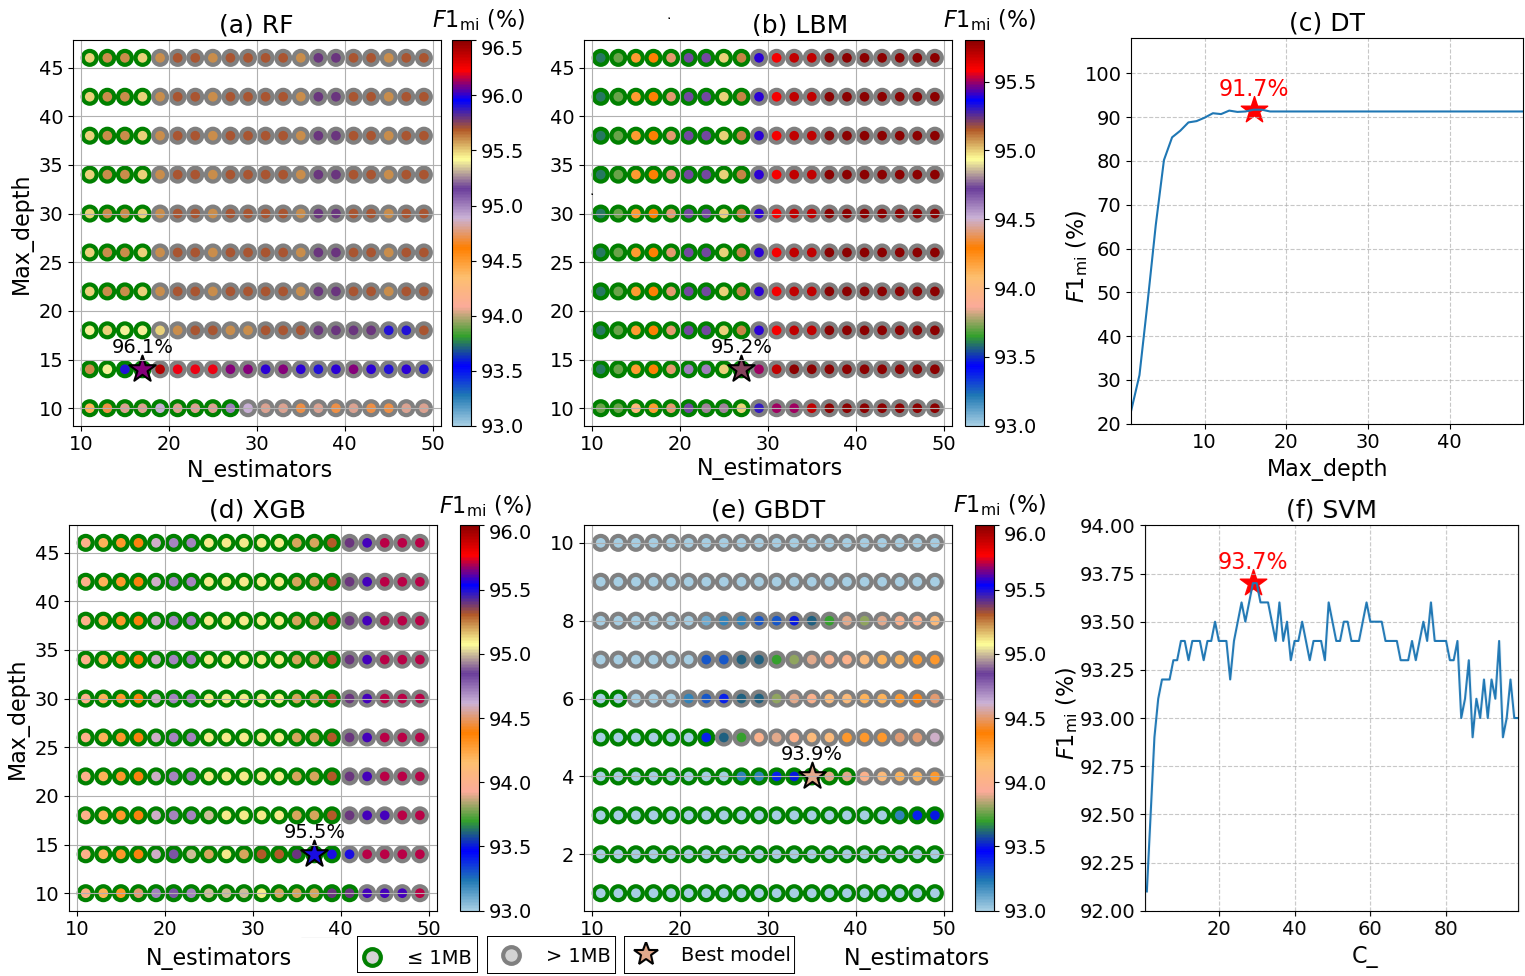
\includegraphics[width=1\linewidth]{Figure/find_parameter.png}
    \caption{Điểm F1$_{mi}$ và kích thước mô hình theo tham số của: (a) RF, (b) LBM, (c) DT, (d) XGB, (e) GBDT, (f) SVM}
    \label{fig:findparam}
\end{figure}

Cấu hình tối ưu của sáu mô hình trên tập dữ liệu riêng được trình bày trong Bảng~\ref{tab:model_config}. Mô hình RF với $n\_\text{estimators} = 17$ và $\text{max\_depth} = 14$ có kích thước 0,9217~MB, thời gian huấn luyện 0,0936~giây và thời gian suy luận 0,0110~giây (tương đương khoảng 3,95~$\mu$s mỗi lần dự đoán).

\begin{table}[!htb]
    \caption{Cấu hình tham số tối ưu các mô hình nhận dạng trên tập dữ liệu riêng}
    \label{tab:model_config}
    \centering
    \footnotesize
    \renewcommand{\arraystretch}{1.2}
    \resizebox{\linewidth}{!}{
    \begin{tabular}{
        >{\arraybackslash}m{0.07\linewidth}
        >{\raggedright\arraybackslash}m{0.28\linewidth}
        >{\centering\arraybackslash}m{0.07\linewidth}
        >{\centering\arraybackslash}m{0.07\linewidth}
        >{\centering\arraybackslash}m{0.07\linewidth}
        >{\centering\arraybackslash}m{0.07\linewidth}
        >{\centering\arraybackslash}m{0.07\linewidth}
        >{\centering\arraybackslash}m{0.07\linewidth}
        >{\centering\arraybackslash}m{0.07\linewidth}
    }
    \hline\hline
    \rowcolor{gray!20}\textbf{Model} & \textbf{Siêu tham số} & $acc$ (\%) & $sen$ (\%) & $spe$ (\%) & $pre$ (\%) & $F1_{mi}$ (\%) & Kích thước (MB) & Trễ (s) \\
    \hline\hline
    RF   & $n{=}17$, $d{=}14$  & 99,3 & 97,0 & 99,6 & 97,1 & \textbf{96,1} & 0,9217 & 0,0110 \\ \hline
    XGB  & $n{=}37$, $d{=}14$  & 99,2 & 96,4 & 99,5 & 96,6 & 95,5 & 0,9398 & 0,0478 \\ \hline
    DT   & $d{=}16$            & 98,5 & 93,3 & 99,1 & 93,6 & 91,7 & 0,0569 & 0,0010 \\ \hline
    GBDT & $n{=}35$, $d{=}4$   & 98,8 & 94,5 & 99,3 & 94,9 & 93,4 & 0,9674 & 0,0149 \\ \hline
    SVM  & $C{=}29$            & 98,9 & 94,8 & 99,4 & 94,6 & 93,7 & 0,2473 & 0,0916 \\ \hline
    LBM  & $n{=}46$, $d{=}22$  & 99,1 & 96,1 & 99,5 & 96,4 & 95,2 & 0,9665 & 0,0080 \\
    \hline\hline
    \end{tabular}}
    \footnotesize \textit{Chú thích: $n$ = số cây; $d$ = độ sâu tối đa; $C$ = tham số điều chuẩn SVM}
\end{table}

\subsubsection{Triển khai TinyML trên vi điều khiển ESP32}

Mô hình RF tối ưu được triển khai trực tiếp trên vi điều khiển ESP32 theo quy trình ba bước:

\textbf{(1) Chuyển đổi và xuất mô hình:} Mô hình đã huấn luyện ($clf$) được chuyển đổi sang mã C thông qua thư viện \texttt{micromlgen}: \texttt{model\_code = port(clf)}, sau đó lưu dưới dạng file header \texttt{random\_forest.h}.

\textbf{(2) Tích hợp mô hình:} File header được nhúng vào firmware vi điều khiển:
\begin{verbatim}
    #include "random_forest.h"
    Eloquent::ml::port::RF rf;
\end{verbatim}

\textbf{(3) Triển khai và thực thi:} Với mỗi vector đặc trưng đầu vào $feat_j$: \texttt{rf.predict(feat\_j)}.

Hình~\ref{fig:suyluan} trình bày thời gian thực tế và thời gian tính toán trên vi điều khiển cho mỗi giai đoạn xử lý. Gia tốc kế lấy mẫu dữ liệu ba trục tại 50~Hz, hệ thống thu thập 150 mẫu trong cửa sổ 3 giây. Sau khi thu thập, trích xuất đặc trưng thực hiện khoảng 8.858~$\mu$s (84.507 dòng lệnh). Mô hình RF với 140.838 dòng lệnh hoàn thành suy luận trong khoảng 733--738~$\mu$s. Tổng độ trễ đầu cuối là xấp xỉ 9.561--9.596~ms.

\begin{figure}[!htb]
    \centering
    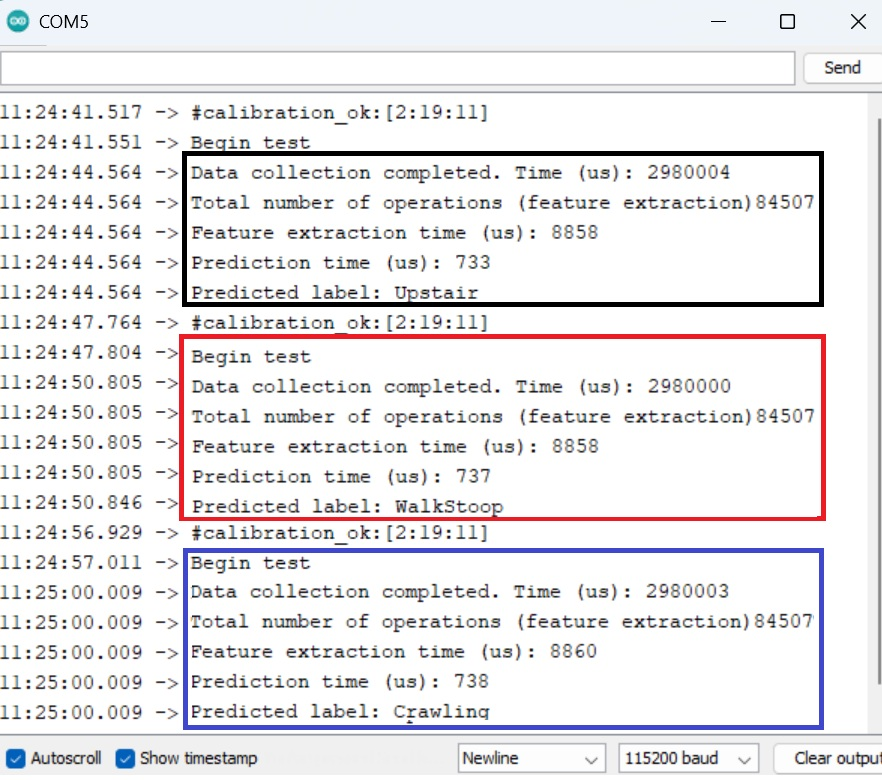
\includegraphics[width=1\linewidth]{Figure/Suyluan.png}
    \caption{Kết quả triển khai dự đoán trên vi điều khiển: thời gian thực tế cho từng giai đoạn xử lý}
    \label{fig:suyluan}
\end{figure}

Mô hình được triển khai là RF gồm 17 cây quyết định, mỗi cây có độ sâu tối đa 14, với kích thước sau biên dịch khoảng 0,92~MB. Độ trễ nhận dạng xấp xỉ 9,561--9,596~ms trên vi điều khiển ESP32, ưu việt hơn một số nghiên cứu liên quan về ứng dụng TinyML trên vi điều khiển \cite{ViManhTuyen2024, Tiny_machine_on_microcontroller, TinyML2023, RIOT_tinyML2025}.

\pagebreak

\section{KẾT QUẢ VÀ THẢO LUẬN}
\label{results_and_discussion}

\subsection{Đánh giá phương pháp định vị}
\label{result_positioning}

\subsubsection{Kết quả thực nghiệm}

\begin{table}[b!]
    \centering
    \caption{Số lượng cửa sổ dữ liệu hướng di chuyển trong NCV trên tập riêng tư}
    \label{nested_cv_direction}
    \begin{tabular}{llrr}\hline\hline
        \textbf{Vòng lặp ngoài (10 fold)} & \textbf{Vòng lặp trong (10 fold)} &  & \textbf{Tổng}\\\hline
        \multirow{2}{*}{Huấn luyện} & Huấn luyện & 2.563 & \multirow{2}{*}{2.848}\\\cline{2-3}
         & Xác thực & 285 & \\\hline
        Kiểm tra &  &  & 317\\\hline
        Tổng &  &  & 3.165\\\hline\hline
    \end{tabular}
\end{table}

\begin{figure}[b!]
    \centering
    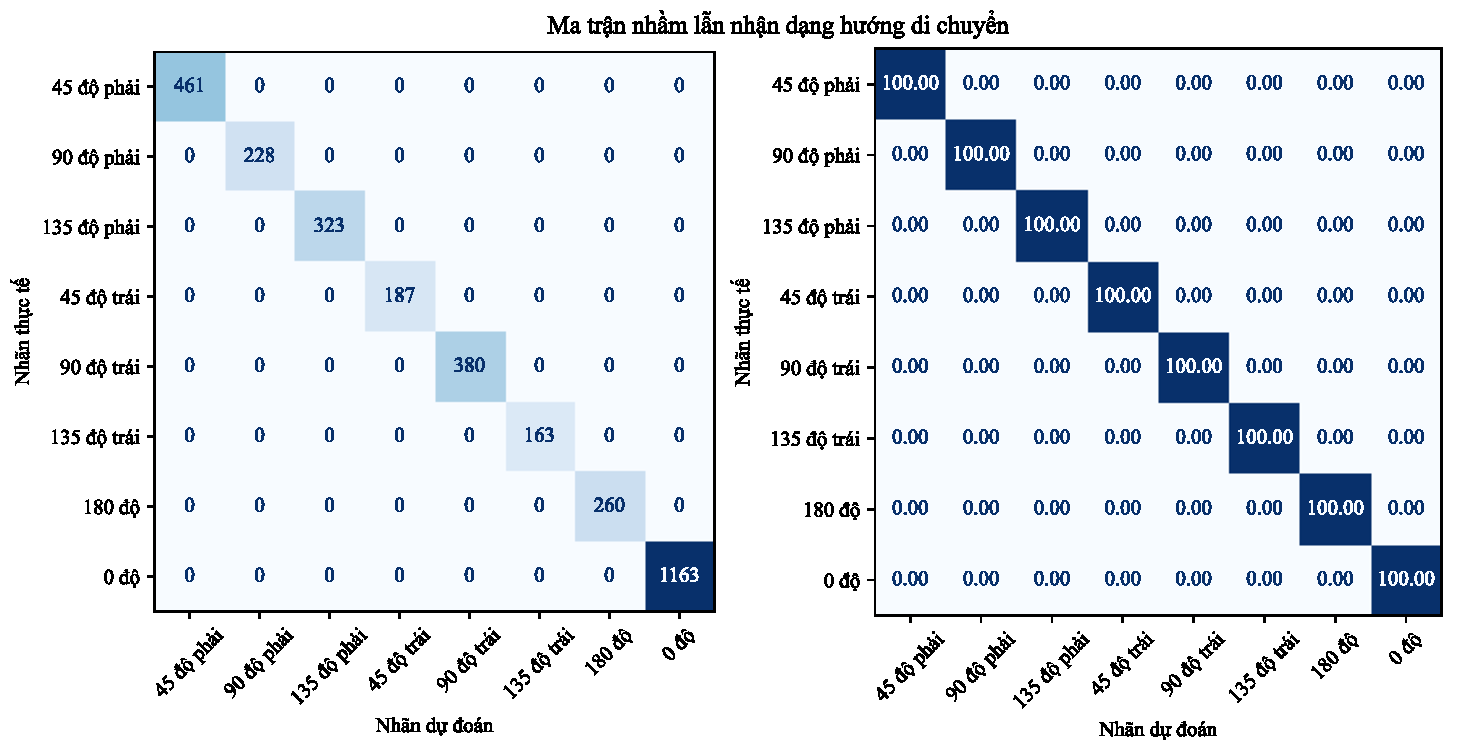
\includegraphics[width=1\linewidth]{Figure/confusion_matrix_direction.pdf}
    \caption{Ma trận nhầm lẫn nhận dạng hướng di chuyển}
    \label{confusion_matrix_direction}
\end{figure}

Để đánh giá hiệu suất của mô hình nhận dạng hướng di chuyển, phương pháp NCV đã được áp dụng nhằm ước lượng sai số tổng quát một cách đáng tin cậy. Cụ thể, kỹ thuật StratifiedKFold được sử dụng trong cả vòng lặp ngoài và vòng lặp trong để xử lý vấn đề mất cân bằng phân bố giữa các lớp dữ liệu. Vòng ngoài gồm 10 fold được sử dụng để đánh giá mô hình, trong khi vòng trong cũng gồm 10 fold nhằm xác định bộ siêu tham số tối ưu cho từng lần lặp ngoài.

Tổng số phân đoạn dữ liệu huấn luyện, xác thực và kiểm tra trong quy trình NCV được trình bày chi tiết trong bảng~\ref{nested_cv_direction}. Quy trình NCV đảm bảo rằng tập kiểm tra hoàn toàn độc lập với tập huấn luyện và xác thực, từ đó giúp giảm thiểu nguy cơ quá khớp và nâng cao độ tin cậy của kết quả. Sau khi hoàn tất quá trình lựa chọn siêu tham số, mô hình được tinh chỉnh thêm bằng quy trình VCV nhằm tối ưu hóa hiệu suất phân loại trên toàn bộ tập dữ liệu huấn luyện.

Mô hình học máy được lựa chọn cuối cùng là DT với độ sâu tối ưu bằng 6 và kích thước bộ nhớ chỉ 3,34 kB. Kết quả phân loại trên toàn bộ cơ sở dữ liệu hướng di chuyển được thể hiện qua ma trận nhầm lẫn trong hình~\ref{confusion_matrix_direction}. Đáng chú ý, mô hình đạt độ chính xác phân loại tuyệt đối $100\%$ trên các lớp hướng di chuyển.

Về mặt tài nguyên triển khai, mô hình có kích thước nhỏ hơn 1 MB, phù hợp với giới hạn bộ nhớ của nhiều vi điều khiển phổ biến hiện nay. Điều này cho thấy rằng các mô hình học máy nhẹ như DT là lựa chọn khả thi cho các ứng dụng nhúng trong thời gian thực, đặc biệt là trong các hệ thống hỗ trợ chiến sĩ cứu hộ, nơi yêu cầu xử lý nhanh với độ trễ thấp và độ tin cậy cao. Việc nhận dạng chính xác hướng di chuyển không chỉ góp phần nâng cao độ chính xác tổng thể của hệ thống định vị, mà còn có ý nghĩa đặc biệt trong việc hỗ trợ giám sát và đảm bảo an toàn cho chiến sĩ trong các tình huống khẩn cấp và môi trường phức tạp.

\begin{figure}[b!]
    \centering
    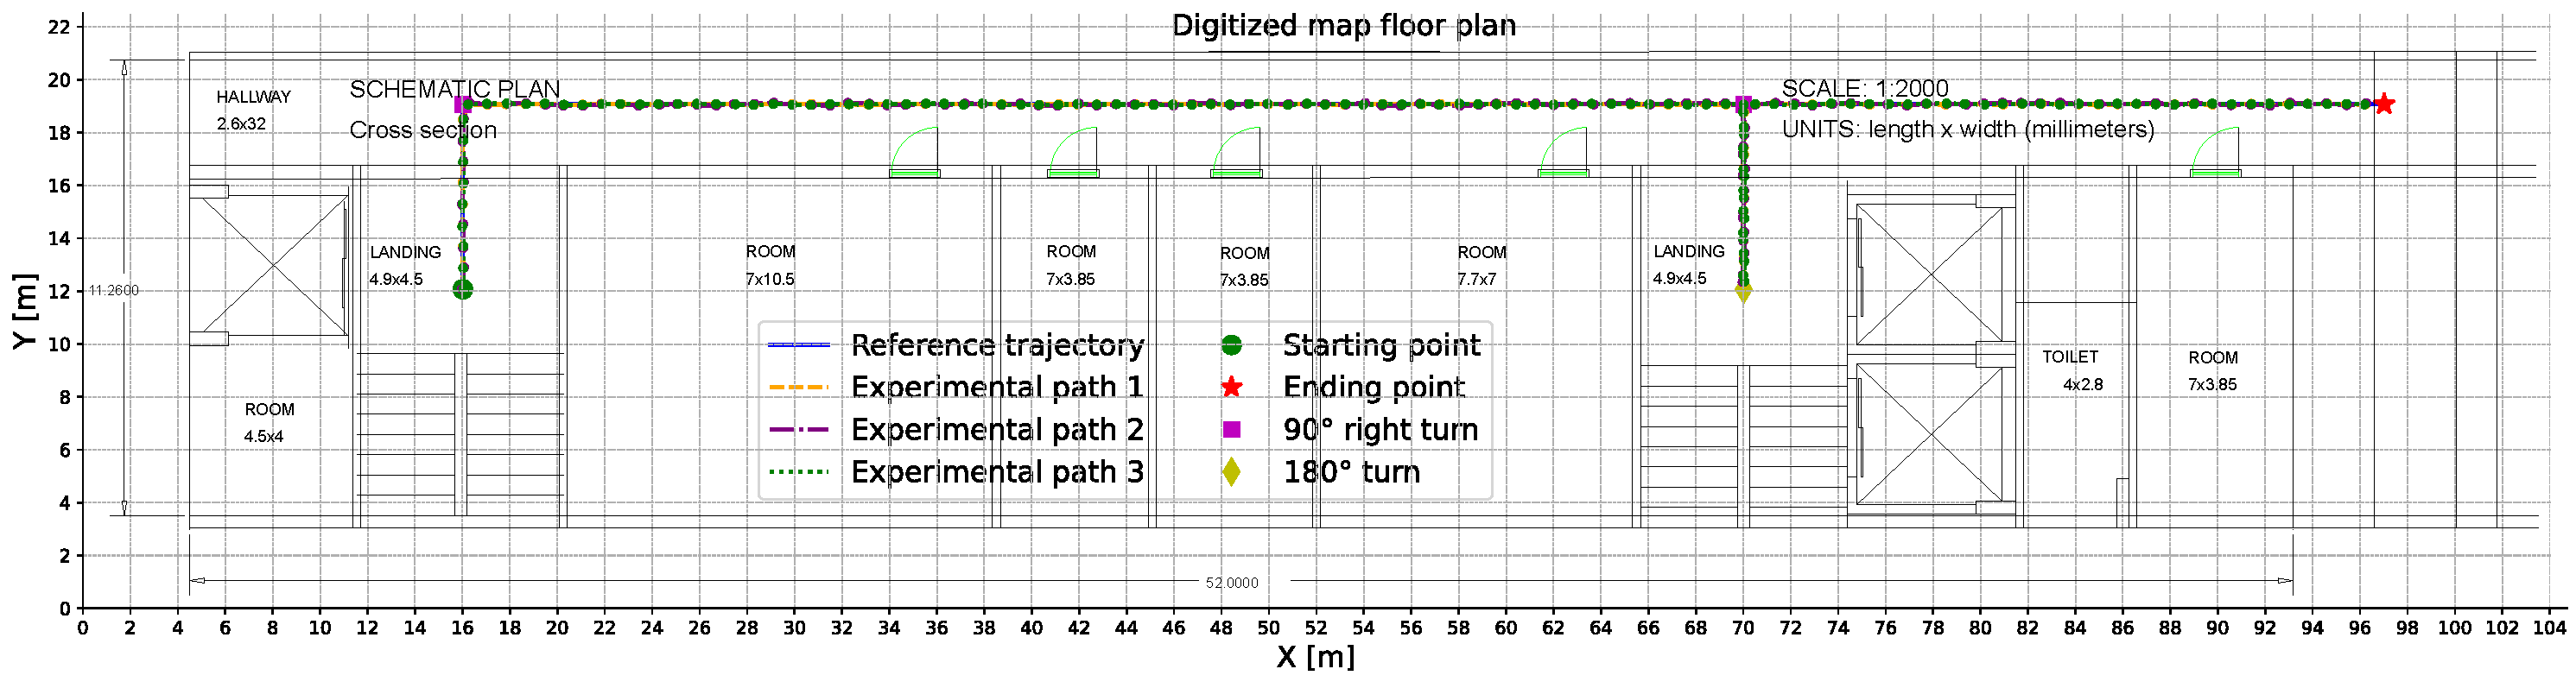
\includegraphics[width=1\linewidth]{Figure/schematic_plane_cross_bold.pdf}
    \caption{Bản đồ số hóa với quỹ đạo tham chiếu và thực nghiệm}
    \label{schematic_plane_cross_bold}
\end{figure}

\begin{table}[b!]
    \centering
    \caption{Khoảng cách ước tính và lỗi trong năm lần thử nghiệm (180 bước, khoảng cách thực tế = 101,5~m)}
    \label{experiment_distance}
    \begin{tabular}{lrrrrr} \hline\hline
    \textbf{Số lần thử nghiệm} & \textbf{1} & \textbf{2} & \textbf{3} & \textbf{4} & \textbf{5} \\ \hline
    Quãng đường ước tính (m) & 101,99 & 102,23 & 101,93 & 102,39 & 100,79\\
    Sai số (m) & 0,49 & 0,73 & 0,43 & 0,89 & 0,71\\ \hline\hline
    \end{tabular}
\end{table}

Trong nghiên cứu này, phương pháp ước tính quãng đường di chuyển được thực hiện dựa trên sự kết hợp giữa bộ đếm bước và phép đo khoảng cách liên chi thông qua LiDAR. Hình ảnh mặt bằng số hóa (Hình~\ref{schematic_plane_cross_bold}) được sử dụng để thiết lập tuyến đường thực nghiệm với kích thước thực tế là 104~m chiều dài và 22,52~m chiều rộng. Để đánh giá độ tin cậy của bộ lọc đa giai đoạn trong việc loại bỏ các vật thể ngoài ý muốn (ví dụ: bức tường, đồ vật), các thử nghiệm được thực hiện trong một hành lang có chiều rộng 2~m, với hai bên là các bức tường. Mỗi lần thử nghiệm bao gồm 180 bước chân, với quãng đường thực tế tương ứng là 101,5~m. Kết quả thực nghiệm cho thấy mô hình ước tính độ dài bước đạt sai số tuyệt đối trung bình 5 cm và độ lệch chuẩn 4,36 cm trên mỗi bước, qua đó đảm bảo tính chính xác của phương pháp ước tính quãng đường di chuyển. Bên cạnh đó, kết quả ước tính quãng đường di chuyển cho từng lần thử nghiệm được trình bày chi tiết trong bảng~\ref{experiment_distance}. Cụ thể, khoảng cách ước tính dao động từ 100,79~m đến 102,39~m, với sai số dao động từ 0,43~m đến 0,89~m. Đáng chú ý, sai số định vị tổng thể của hệ thống luôn duy trì dưới 2~m trong tất cả các thử nghiệm, khẳng định tính hiệu quả và độ tin cậy của phương pháp đề xuất. Điều này là một lợi thế quan trọng đối với các ứng dụng trong môi trường cứu hộ khẩn cấp trong nhà, nơi yêu cầu cao về tính chính xác và khả năng theo dõi liên tục.

Tuy nhiên, phương pháp ước tính quãng đường di chuyển sử dụng LiDAR chỉ thực sự khả thi trong các trạng thái di chuyển đi bộ hoặc đi nhanh—tức là khi đối tượng di chuyển đều và luôn có ít nhất một chân chạm đất. Trong trường hợp đối tượng chuyển sang trạng thái chạy bộ, cả hai chân có thể đồng thời không chạm đất, dẫn đến gián đoạn trong phép đo khoảng cách của LiDAR. Do đó, trong tình huống chạy bộ, hệ thống chỉ có thể dựa vào bộ đếm bước để ước tính quãng đường di chuyển, trong khi các phép đo từ LiDAR có thể bị loại bỏ hoặc không đáng tin cậy do sự bất ổn định trong dữ liệu quét. Nhìn chung, các kết quả thực nghiệm đã chứng minh tính khả thi và hiệu quả của phương pháp tích hợp LiDAR và bộ đếm bước trong việc ước tính quãng đường di chuyển của đối tượng trong môi trường trong nhà. Tuy nhiên, để mở rộng ứng dụng cho các tình huống phức tạp hơn như chạy bộ, bò trườn, cần có các phương pháp hiệu chỉnh và điều chỉnh thuật toán nhằm đảm bảo tính chính xác và ổn định của hệ thống.

\subsubsection{Thảo luận các phương pháp định vị nhân viên cứu hộ trong nhà}

\begin{figure}[t]
    \centering
    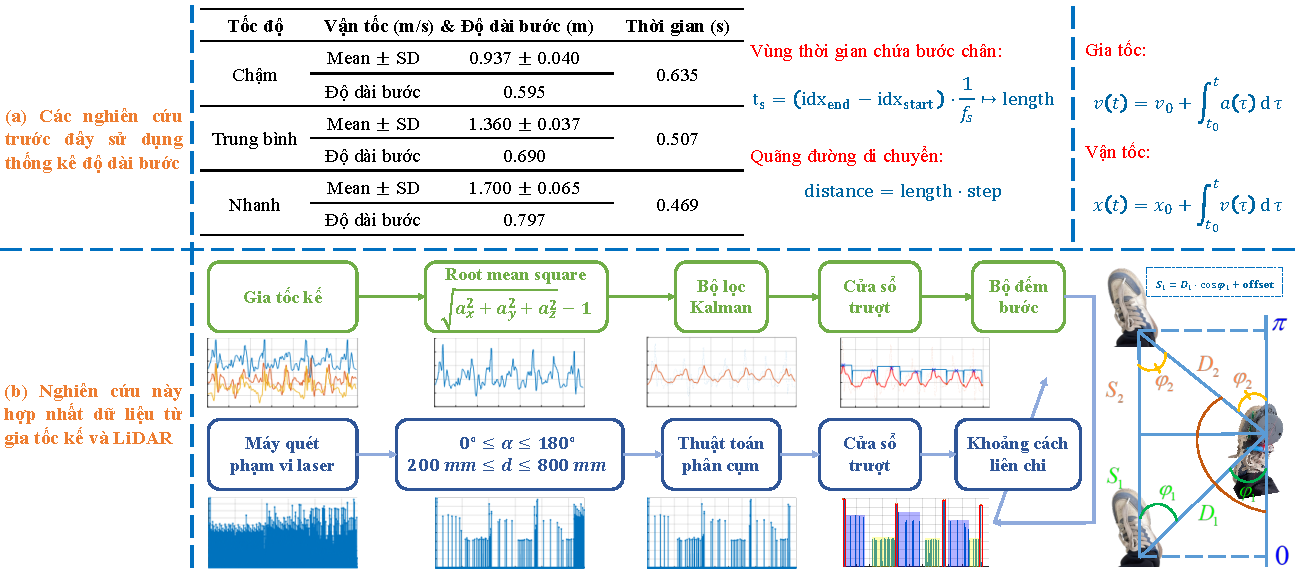
\includegraphics[width=1\linewidth]{Figure/discussion_ips.pdf}
    \caption{So sánh giữa (a) Phương pháp ước lượng quãng đường di chuyển dựa trên thống kê độ dài bước trong các nghiên cứu trước đây~\cite{pham2018highly}, \cite{ho2016step} và (b) Chiến lược hợp nhất cảm biến IMU-LiDAR đề xuất trong nghiên cứu này}
    \label{discussion_estimate}
\end{figure}

Trong các nghiên cứu trước đây, việc ước tính quãng đường di chuyển thường dựa vào việc đếm số bước kết hợp với bảng tra thống kê độ dài bước tương ứng với từng mức tốc độ (chậm, trung bình, nhanh)~\cite{pham2018highly}, \cite{ho2016step}. Phương pháp này giả định rằng độ dài bước chân là hằng số đối với mỗi người tại mỗi tốc độ, từ đó nhân với số bước để tính quãng đường (Hình~\ref{discussion_estimate}a). Tuy nhiên, giả định này khó phản ánh chính xác chuyển động thực tế vì độ dài bước phụ thuộc vào nhiều yếu tố như thể trạng, dáng đi, tải trọng mang theo, trạng thái mệt mỏi hoặc đặc thù thao tác của lính cứu hỏa trong điều kiện khẩn cấp.

Nhằm khắc phục nhược điểm trên, nghiên cứu này đề xuất một phương pháp hợp nhất dữ liệu từ cảm biến quán tính (IMU) và máy quét phạm vi laser (LiDAR) thông qua một kiến trúc bộ lọc đa giai đoạn, nhằm ước lượng chính xác quãng đường di chuyển theo thời gian thực (Hình~\ref{discussion_estimate}b). Cụ thể, bộ đếm bước sử dụng tín hiệu gia tốc từ IMU giúp xác định chính xác thời điểm diễn ra từng bước chân. Thông tin này đóng vai trò là tín hiệu khởi phát cho thuật toán phát hiện đỉnh từ dữ liệu LiDAR, vốn được xử lý qua ba tầng lọc: giới hạn phạm vi quét, phân cụm để loại bỏ nhiễu, và cửa sổ trượt để phát hiện đỉnh tương ứng với khoảng cách giữa hai bàn chân.

Cách tiếp cận này mang lại hai lợi ích quan trọng. Thứ nhất, nó loại bỏ được các bước chân giả do dao động nhiễu hoặc vật thể ngoài vùng quan tâm trong dữ liệu LiDAR. Thứ hai, nó đảm bảo rằng chỉ các bước chân hợp lệ mới được đưa vào tính toán, từ đó giúp cải thiện độ chính xác trong ước lượng độ dài bước. Việc sử dụng thông tin đo trực tiếp thay vì dựa trên bảng tra cứu giúp hệ thống thích ứng linh hoạt với hành vi chuyển động thực tế của từng cá nhân trong nhiều tình huống khác nhau—điều đặc biệt quan trọng trong môi trường khẩn cấp như tìm kiếm cứu nạn. Tóm lại, phương pháp đề xuất không chỉ cải thiện độ chính xác định vị so với cách tiếp cận truyền thống mà còn có tính thích nghi cao và khả năng ứng dụng thực tiễn trong các kịch bản khắc nghiệt. Hệ thống cho thấy tiềm năng lớn trong việc hỗ trợ giám sát và điều phối chiến sĩ cứu nạn trong các tòa nhà bị ảnh hưởng bởi hỏa hoạn, nơi các công nghệ định vị dựa trên hạ tầng gần như không thể hoạt động ổn định.

\begin{table}[t]
    \centering
    \caption{So sánh các phương pháp định vị nhân viên cứu hộ trong nhà tiêu biểu cho các tình huống khẩn cấp}
    \label{discussion_ips}
    \begin{tabular}{p{0.09\linewidth}p{0.151\linewidth}p{0.2\linewidth}p{0.186\linewidth}p{0.24\linewidth}}\hline\hline
        \multicolumn{1}{c}{\textbf{Ấn phẩm}} & \multicolumn{1}{c}{\textbf{Công nghệ}} & \multicolumn{1}{c}{\textbf{Phương pháp}} & \multicolumn{1}{c}{\textbf{Kỹ thuật}} & \multicolumn{1}{c}{\textbf{Sai số và thách thức}}\\\hline

        \multirow{8}{*}{\parbox[t]{\linewidth}{\justifying \noindent Nghiên cứu này}} & \multirow{8}{*}{\parbox[t]{\linewidth}{\justifying \noindent IMU 6-DoF, khí áp kế (thắt lưng) và LiDAR (bàn chân)}} & \makecell[tl]{\parbox[t]{\linewidth}{\justifying \noindent - IMU đếm bước + sải chân từ LiDAR giữa các chân.\\- 8 lớp HAR và 8 lớp di chuyển.\\- Ước tính độ cao từ khí áp kế kết hợp IMU và HAR.}} & \multirow{8}{*}{\makecell[tl]{\parbox[t]{\linewidth}{\justifying \noindent - Lọc LiDAR 3 giai đoạn.\\- XGBoost cho HAR.\\- DT cho hướng di chuyển.\\- Bộ lọc Kalman.}}} & \multirow{8}{*}{\makecell[tl]{\parbox[t]{\linewidth}{\justifying \noindent - HAR 98,38~\%, hướng di chuyển 100~\%.\\ - Lỗi định vị $<$ 2~m.\\- Ổn định trong trạng thái đi bộ.\\ - Tắc nghẽn LiDAR, biến đổi áp suất.}}} \\
        \hline
        
        \multirow{6}{*}{\makecell[tl]{Yuan \\ \textit{et al.}~\cite{yuan2016research}}} & \multirow{6}{*}{\parbox[t]{\linewidth}{\justifying \noindent IMU 6-DoF (bàn chân)}} & \multirow{6}{*}{\makecell[tl]{\parbox[t]{\linewidth}{\justifying \noindent - Tính khoảng cách và độ cao bằng gia tốc kế.\\- Xác định hướng bằng con quay hồi chuyển.}}} & \multirow{6}{*}{\makecell[tl]{\parbox[t]{\linewidth}{\justifying \noindent - Tích phân kép INS: \\ $p_n = \int v_n\,dt = \int (a_n + g_t)\,dt$.\\- Tối ưu hóa rời rạc và ZUPT.}}} & \makecell[tl]{\parbox[t]{\linewidth}{\justifying \noindent - Sai số tương đối $<$ 1~\% (sai số tuyệt đối lên tới 2,5~m).\\- Độ trôi tích lũy theo thời gian.\\- Biến thiên dáng đi.}} \\
        \hline
        
        \multirow{10}{*}{\makecell[tl]{Cinaz và \\ Kenn~\cite{cinaz2008headslam}}} & \multirow{10}{*}{\parbox[t]{\linewidth}{\justifying \noindent IMU 6-DoF và máy quét laser (gắn đầu)}} & \multirow{10}{*}{\makecell[tl]{\parbox[t]{\linewidth}{\justifying \noindent - Định vị và lập bản đồ đồng thời (SLAM).\\- Laser quét hiệu chỉnh theo hướng đầu (IMU).\\- Vận tốc bước giả định từ IMU.}}} & \multirow{10}{*}{\makecell[tl]{\parbox[t]{\linewidth}{\justifying \noindent - Bộ lọc hạt Rao-Blackwellized (GMapping).\\- Ước lượng bước từ dao động trục Z.\\- Biến đổi góc 3D thành mặt phẳng quét.}}} & \makecell[tl]{\parbox[t]{\linewidth}{\justifying \noindent - 0,7~m trong phòng có vật cản.\\- 6 đến 12~m trong hành lang mở.\\- 18~m trong hành lang trống.\\- Phụ thuộc đặc trưng môi trường.\\- Lỗi do chuyển động đầu phức tạp.}} \\
        \hline
        
        \multirow{5}{*}{\makecell[tl]{De \\ \textit{et al.}~\cite{de2017hybrid}}} & \multirow{5}{*}{\parbox[t]{\linewidth}{\justifying \noindent IMU 9-DoF (thắt lưng) và thẻ RFID thụ động}} & \makecell[tl]{\parbox[t]{\linewidth}{\justifying \noindent - IMU ước lượng chuyển động.\\- RFID sửa lỗi trôi.\\- RFID cài sẵn trong đèn báo khẩn cấp.}} & \makecell[tl]{\parbox[t]{\linewidth}{\justifying \noindent - Vi phân quaternion: \\ $\frac{d\mathbf{q}}{dt} = \boldsymbol{\Omega} \mathbf{q}$.\\- Bộ lọc định hướng Kalman mở rộng.\\ - Bộ lọc Bayesian.}} & \multirow{5}{*}{\makecell[tl]{\parbox[t]{\linewidth}{\justifying \noindent - Sai số $<$ 4~m với PDR; $<$ 2.6~m với hệ lai.\\- Từ kế bị nhiễu.\\- Thẻ RFID có thể hư hỏng.}}} \\\hline\hline
    \end{tabular}
\end{table}

Bên cạnh các phương pháp thống kê truyền thống trong ước lượng quãng đường, nhiều nghiên cứu trong lĩnh vực định vị lính cứu hỏa cũng khai thác các kỹ thuật cảm biến đeo không phụ thuộc hạ tầng để đảm bảo tính tự chủ và khả năng triển khai trong môi trường khẩn cấp. Bảng~\ref{discussion_ips} định vị cách tiếp cận của chúng tôi so với các phương pháp định vị trong nhà tiêu biểu gồm: định vị quán tính thuần túy, định vị dựa trên SLAM với máy quét laser đeo đầu, và định vị lai IMU-RFID.

Yuan \textit{et al.}~\cite{yuan2016research} đề xuất một hệ thống định vị độc lập hoàn toàn dựa trên IMU gắn ở bàn chân, kết hợp thuật toán phát hiện bước, ước lượng vận tốc và hiệu chỉnh bằng kỹ thuật ZUPT. Nhờ xác định chính xác thời điểm chân đứng yên, hệ thống có thể hạn chế sai số tích lũy khi tích phân vận tốc. Thử nghiệm thực tế với các tình huống đa dạng (đi bộ, chạy, leo cầu thang, địa hình đổ nát) cho thấy sai số tương đối thấp (khoảng $<$ 1~\%, sai số tuyệt đối lên đến 2,5~m) trên các hành trình ngắn và vừa. Tuy nhiên, khi kéo dài thời gian hoạt động, hệ thống vẫn gặp vấn đề với trôi tích lũy, đặc biệt trong điều kiện không có thông tin hiệu chỉnh từ bản đồ hay hạ tầng. Ngoài ra, hướng chuyển động dễ bị sai lệch nếu không có hỗ trợ từ cảm biến từ trường hoặc các mô hình bổ sung.

Cinaz và Kenn~\cite{cinaz2008headslam} với hệ thống HeadSLAM kết hợp IMU và máy quét laser gắn trên đầu nhằm thực hiện đồng thời định vị và lập bản đồ môi trường 2D thông qua thuật toán SLAM dựa trên bộ lọc hạt Rao-Blackwellized. Phương pháp này có ưu điểm lớn là không phụ thuộc vào bản đồ có sẵn hay hạ tầng định vị, đồng thời tận dụng kỹ thuật scan matching để tăng cường khả năng xác định vị trí trong thời gian thực. Tuy nhiên, sai số định vị tăng đáng kể trong môi trường hành lang đơn điệu hoặc không có vật cản đặc trưng, với độ lệch có thể lên đến 18~m (cụ thể 0,7~m trong phòng có vật cản, 6 đến 12~m trong hành lang mở, 18~m trong hành lang trống). Hạn chế chủ yếu nằm ở việc quét laser bị ảnh hưởng mạnh bởi hướng chuyển động đầu, chuyển động holonomic không ổn định, và không có cơ chế đóng vòng hiệu quả—điều vốn rất quan trọng trong các hành trình dài hoặc khép kín.

De Cillis \textit{et al.}~\cite{de2017hybrid} đề xuất hệ thống lai IMU-RFID với chiến lược hiệu chỉnh vị trí dựa trên thông tin định vị tích hợp trong thẻ RFID cài sẵn tại các vị trí chiến lược trong tòa nhà. Với thiết kế bộ lọc Bayes hai pha: pha dự đoán dựa trên bước đi PDR từ dữ liệu quán tính và pha hiệu chỉnh dựa trên thông tin ngữ cảnh được trích xuất từ thẻ RFID gắn sẵn tại các vị trí chiến lược, hệ thống có thể duy trì sai số định vị dưới 2,6~m kể cả trong hành trình kéo dài, miễn là thẻ RFID không bị phá hủy hoặc mất tín hiệu và dưới 4~m chỉ với PDR. Tuy vậy, việc phụ thuộc vào các nút RFID khiến hệ thống dễ bị ảnh hưởng nếu thẻ bị hỏng, lắp sai hoặc không đủ mật độ phủ. Bên cạnh đó, không giống như cảm biến gắn ở bàn chân, IMU gắn thắt lưng không cho phép áp dụng các kỹ thuật ZUPT, từ đó làm tăng rủi ro tích lũy sai số khi di chuyển liên tục mà không có hiệu chỉnh.

So với các nghiên cứu trên, phương pháp đề xuất trong nghiên cứu này lựa chọn chiến lược hợp nhất IMU-LiDAR với kiến trúc lọc ba tầng, đồng thời khai thác vị trí lắp đặt cảm biến hợp lý (IMU tại thắt lưng và LiDAR tại bàn chân phải) để trực tiếp đo khoảng cách giữa hai chân—qua đó tính toán độ dài bước trong thời gian thực thay vì dựa vào bảng thống kê. Cách tiếp cận này không chỉ đảm bảo độ chính xác cao ($<$ 2~m) trong hành trình tuyến tính mà còn cải thiện khả năng thích nghi với thay đổi tư thế, sải chân và trạng thái hoạt động của lính cứu hỏa. Hệ thống cũng cho thấy khả năng triển khai thực tế cao nhờ kích thước mô hình nhỏ, dễ nhúng và không yêu cầu bất kỳ hạ tầng bên ngoài nào. Nhờ đó, phương pháp đề xuất đã khắc phục được hạn chế quan trọng của các nghiên cứu trước: hoặc chưa có biện pháp hiệu chỉnh sai số tích lũy theo thời gian (Yuan \textit{et al.}~\cite{yuan2016research}), hoặc phụ thuộc vào môi trường (HeadSLAM~\cite{cinaz2008headslam}, De Cillis \textit{et al.}~\cite{de2017hybrid}).

Tổng thể, sự kết hợp giữa đặc trưng động học từ IMU, phép đo vật lý chính xác từ LiDAR, và bộ lọc đa tầng xử lý dữ liệu đầu vào, đã giúp hệ thống đề xuất trở thành một giải pháp cân bằng giữa độ chính xác, tính tự chủ và khả năng triển khai trong môi trường nguy hiểm, vốn là yêu cầu cốt lõi trong bài toán định vị lính cứu nạn trong nhà. Những lợi ích bắt nguồn từ ước tính bước chân LiDAR giữa các chân và khí áp kế hỗ trợ độ cao, giúp hạn chế độ trôi mà không cần đèn hiệu môi trường. Các hạn chế bao gồm tắc nghẽn LiDAR và các biến đổi áp suất; công việc trong tương lai sẽ nhắm mục tiêu vào các đường dẫn dài hơn, các đoạn rẽ gấp và chuyển đổi nhiều tầng thông qua sự kết hợp mạnh mẽ hơn.


\subsection{Đánh giá phương pháp nhận dạng hành động}
\label{result_har}

\subsubsection{Kết quả trên các bộ dữ liệu thử nghiệm}

\paragraph{Đánh giá trên tập dữ liệu riêng tư}

\begin{figure}[b!]
    \centering
    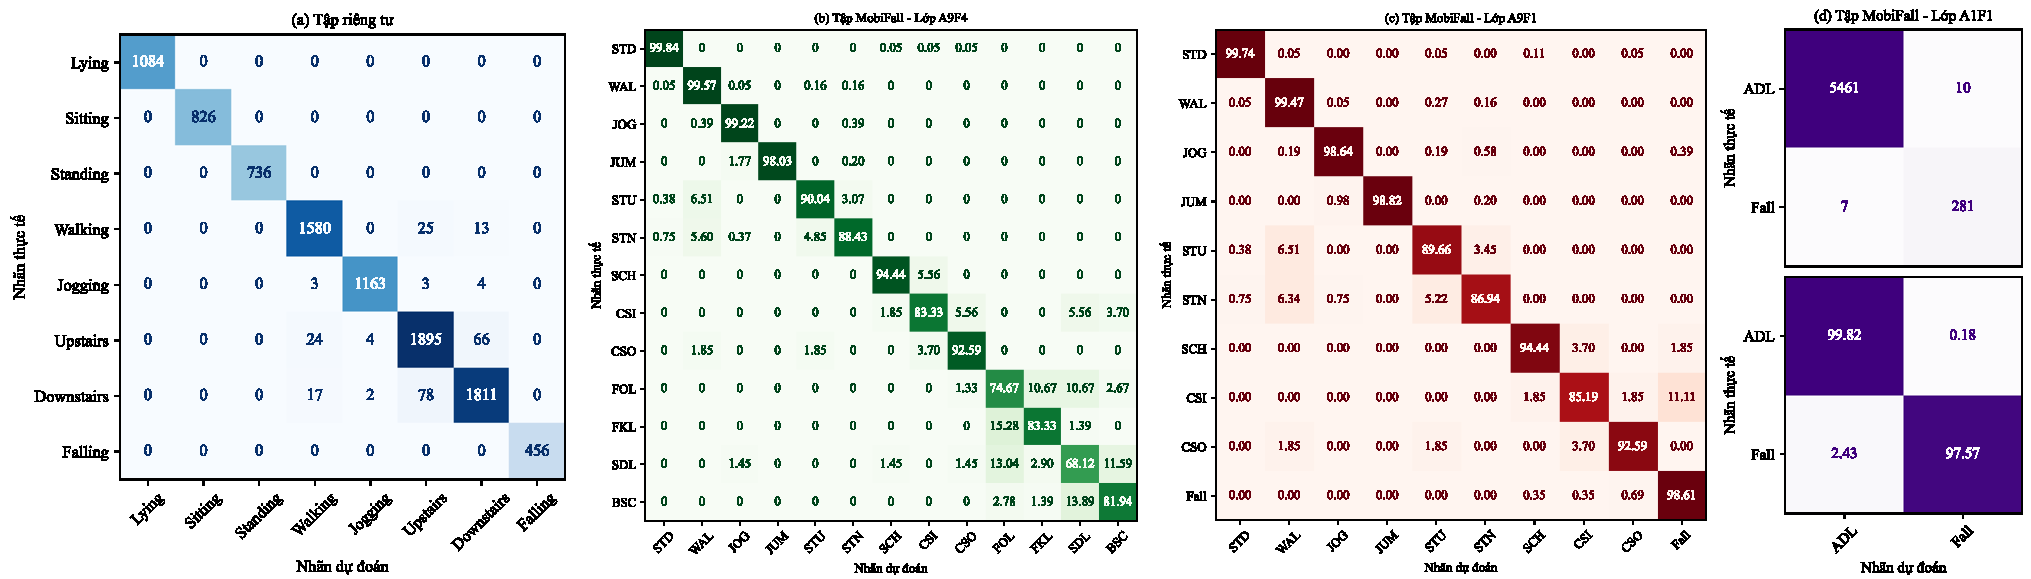
\includegraphics[width=1\linewidth]{Figure/confusion_matrices.pdf}
    \caption{Ma trận nhầm lẫn trên toàn bộ cơ sở dữ liệu: (a) Tập riêng tư; Tập MobiFall với (b) Tổ hợp A9F4, (c) Tổ hợp A9F1 và (d) Tổ hợp A1F1}
    \label{confusion_matrices}
\end{figure}

\begin{table}[t]
    \centering
    \caption{Báo cáo kết quả phân loại trên tập riêng tư và các tổ hợp A9F4, A9F1 trên tập MobiFall}
    \label{classification_report}
    \begin{tabular}{lccc||cccc||cccc}\hline\hline
        \multicolumn{4}{c||}{\textbf{Tập riêng tư}} & \multicolumn{4}{c||}{\textbf{Tập MobiFall - Tổ hợp A9F4}} & \multicolumn{4}{c}{\textbf{Tập MobiFall - Tổ hợp A9F1}}\\
        \textbf{Activity} & \textbf{PRE} & \textbf{SEN} & \textbf{F1} & \textbf{Activity} & \textbf{PRE} & \textbf{SEN} & \textbf{F1} & \textbf{Activity} & \textbf{PRE} & \textbf{SEN} & \textbf{F1}\\\hline
        Lying & 100 & 100 & 100 & STD & 99,79 & 99,84 & 99,81 & STD & 99,79 & 99,74 & 99,76\\
        
        Sitting & 100 & 100 & 100 & WAL & 98,16 & 99,57 & 98,86 & WAL & 98,05 & 99,47 & 98,75\\
        
        Standing & 100 & 100 & 100 & JOG & 97,70 & 99,22 & 98,46 & JOG & 98,45 & 98,64 & 98,54\\
        
        Walking & 97,29 & 97,65 & 97,47 & JUM & 100 & 98,03 & 99,01 & JUM & 100 & 98,82 & 99,41\\
        
        Jogging & 99,49 & 99,15 & 99,32 & STU & 93,25 & 90,04 & 91,62 & STU & 91,41 & 89,66 & 90,52\\
        
        Upstairs & 94,70 & 95,27 & 94,99 & STN & 94,42 & 88,43 & 91,33 & STN & 93,57 & 86,94 & 90,14\\
        
        Downstairs & 95,62 & 94,92 & 95,27 & SCH & 94,44 & 94,44 & 94,44 & SCH & 92,73 & 94,44 & 93,58\\
        
        Falling & 100 & 100 & 100 & CSI & 88,24 & 83,33 & 85,71 & CSI & 90,20 & 85,19 & 87,62\\
        
         &  &  &  & CSO & 89,29 & 92,59 & 90,91 & CSO & 92,59 & 92,59 & 92,59\\
         
         &  &  &  & FOL & 71,79 & 74,67 & 73,20 & Fall & 96,93 & 98,61 & 97,76\\
         
         &  &  &  & FKL & 84,51 & 83,33 & 83,92 &  &  &  & \\
         &  &  &  & SDL & 68,12 & 68,12 & 68,12 &  &  &  & \\
         &  &  &  & BSC & 83,10 & 81,94 & 82,52 &  &  &  & \\\hline\hline
    \end{tabular}
\end{table}

\begin{table}[t]
    \centering
    \caption{Đánh giá hiệu suất mô hình trên tập MobiFall với ba kỹ thuật xác thực chéo và ba cấu hình tổ hợp}
    \label{cross_validation_techniques}
    \begin{tabular}{ccccccc}\hline\hline
        \multirow{2}{*}{\textbf{MobiFall}} 
        & \multicolumn{2}{c}{\textbf{K-Fold}} 
        & \multicolumn{2}{c}{\textbf{Leave-One-Subject-Out\textsuperscript{$\flat$}}} 
        & \multicolumn{2}{c}{\textbf{Leave-Recordings-Out\textsuperscript{$\dag$}}} \\\cline{2-7}
         & \textbf{Accuracy} & \textbf{F1\textsubscript{macro}} 
         & \textbf{Accuracy} & \textbf{F1\textsubscript{macro}} 
         & \textbf{Accuracy} & \textbf{F1\textsubscript{macro}} \\\hline
        A9F4 & 97,15 $\pm$ 0,67 & 88,93 $\pm$ 2,29 & 80,26 $\pm$ 13,54 & 73,93 $\pm$ 16,81 & 88,64 $\pm$ 8,72 & 80,29 $\pm$ 4,19\\\hline
        A9F1 & 98,11 $\pm$ 0,68 & 94,72 $\pm$ 2,66 & 92,86 $\pm$ 11,02 & 86,19 $\pm$ 19,39 & 88,99 $\pm$ 7,71 & 82,96 $\pm$ 5,61\\\hline
        A1F1 & 99,70 $\pm$ 0,16 & 98,44 $\pm$ 0,84 & \hspace{-0.5em}98,31 $\pm$ 3,94 & 90,97 $\pm$ 17,64 & 99,58 $\pm$ 0,43 & 98,76 $\pm$ 0,85\\\hline\hline
    \end{tabular}
\vspace{0.2em}\\
\noindent \textsuperscript{$\flat$}24 chủ thể, \textsuperscript{$\dag$}99 bản ghi
\end{table}

Hiệu suất của mô hình XGBoost được xác nhận thông qua quy trình NCV, với điểm F1\textsubscript{macro} đạt 98,38 $\pm$ 0,40~\%. Khi áp dụng mô hình lên toàn bộ tập dữ liệu riêng tư, kết quả được thể hiện trong hình~\ref{confusion_matrices}a và bảng~\ref{classification_report}. Mô hình cho thấy khả năng phân loại chính xác tuyệt đối (100~\%) đối với các hành động tĩnh như nằm, ngồi, đứng, cũng như hành động ngã. Đây là các hành vi có đặc trưng động học ổn định và rõ ràng, giúp mô hình dễ dàng nhận diện trong không gian đặc trưng đã được trích xuất.

Ngược lại, độ chính xác giảm nhẹ ở các hành động vận động, đặc biệt là các hành vi có đặc điểm dao động chu kỳ như đi bộ (1.580/1.618, 97,65~\%), chạy bộ (1.163/1.173, 99,15~\%), lên cầu thang (1.895/1.989, 95,27~\%) và xuống cầu thang (1.811/1.908, 94,92~\%). Như đã phân tích trước đó qua biểu đồ histogram và biểu diễn t-SNE, các hành vi này có dạng phân bố tín hiệu tương tự nhau cả về biên độ và chu kỳ dao động, dẫn đến hiện tượng chồng lấp trong không gian đặc trưng. Hiện tượng này cũng đã được ghi nhận trong nghiên cứu của Vi \textit{et al.}~\cite{vi2024efficient}, khi nhóm tác giả quyết định hợp nhất hai hành động lên và xuống cầu thang thành một lớp duy nhất để giảm nhầm lẫn và cải thiện độ chính xác tổng thể.

Tóm lại, kết quả đạt được trên tập dữ liệu riêng tư không chỉ phản ánh hiệu suất cao của mô hình mà còn phù hợp với phân tích định tính về đặc trưng tín hiệu. Những quan sát này đóng vai trò quan trọng trong việc giải thích hành vi mô hình, đồng thời cung cấp căn cứ để điều chỉnh chiến lược phân loại trong các nghiên cứu tiếp theo.

\paragraph{Đánh giá trên tập dữ liệu công khai MobiFall}

Bộ dữ liệu MobiFall bao gồm tổng cộng 13 loại hoạt động, trong đó có 9 hành động thường ngày và 4 hành động ngã. Nhằm đánh giá hiệu suất mô hình nhóm nghiên cứu đề xuất một cách toàn diện và tương thích với các phương pháp phân loại phổ biến trong cộng đồng nghiên cứu, chúng tôi thực hiện đánh giá trên ba cấu hình tổ hợp hành động khác nhau:

\begin{boxlabel}
    \item Tổ hợp A9F4: Gồm đầy đủ 9 hành động thường ngày và 4 hành động ngã—tương ứng với bài toán phân loại 13 lớp.

    \item Tổ hợp A9F1: Giữ nguyên 9 hành động thường ngày, trong khi gộp toàn bộ các hành động ngã vào một lớp duy nhất—phù hợp với nhiều ứng dụng phát hiện ngã trong môi trường thực tế.

    \item Tổ hợp A1F1: Gộp toàn bộ ADL thành một lớp duy nhất là “không ngã”, và so sánh với lớp “ngã”—tương ứng với bài toán nhị phân phổ biến trong các nghiên cứu phát hiện ngã.
\end{boxlabel}

Để đánh giá hiệu suất tổng quát và khả năng triển khai thực tế của mô hình trên dữ liệu chưa từng thấy, chúng tôi áp dụng ba chiến lược xác thực chéo khác nhau trên tập dữ liệu MobiFall: (i) xác thực chéo $k$-fold, (ii) xác thực chéo để lại từng chủ thể (Leave-One-Subject-Out) và (iii) xác thực chéo để lại từng bản ghi (Leave-Recordings-Out). Mỗi phương pháp cung cấp một góc nhìn khác nhau về năng lực khái quát hóa của mô hình, từ đó cho phép đánh giá toàn diện hiệu quả phân loại trong các kịch bản ứng dụng khác nhau.

% \begin{enumerate}[label=(\roman*)]
%     \item Xác thực chéo $k$-fold: Tập dữ liệu MobiFall được chia thành 10 phần bằng nhau (folds). Mỗi lần lặp, một phần được giữ lại để kiểm thử trong khi chín phần còn lại được dùng để huấn luyện. Quá trình này được lặp lại đủ 10 lần với mỗi phần lần lượt đóng vai trò kiểm thử. Cách tiếp cận này duy trì được sự cân bằng giữa dữ liệu huấn luyện và kiểm thử, đồng thời cung cấp trung bình hiệu suất mô hình đáng tin cậy.

%     \item Xác thực chéo để lại từng chủ thể (Leave-One-Subject-Out): Với tổng số 24 tình nguyện viên tham gia, phương pháp này thực hiện huấn luyện mô hình trên dữ liệu từ 23 người và đánh giá trên người còn lại. Quá trình này được lặp lại cho tất cả các chủ thể, đảm bảo rằng mỗi người đều được giữ lại một lần cho kiểm thử. Đây là tiêu chí đánh giá nghiêm ngặt nhất về năng lực khái quát hóa của mô hình khi gặp dữ liệu từ người hoàn toàn mới—điều đặc biệt quan trọng trong các ứng dụng triển khai thực tế với người dùng mới.

%     \item Xác thực chéo theo bản ghi (Leave-Recordings-Out): Mỗi bản ghi tương ứng với một phiên thu liên tục từ khi bắt đầu đến khi kết thúc một hành động. Tập dữ liệu MobiFall bao gồm tổng cộng 99 bản ghi. Chúng tôi áp dụng chiến lược xác thực chéo theo nhóm với k $=$ 10, trong đó mỗi fold chứa khoảng 10 bản ghi được giữ lại làm tập kiểm thử, các bản ghi còn lại dùng để huấn luyện. Cách làm này cho phép đánh giá khả năng khái quát hóa của mô hình khi gặp các đoạn dữ liệu mới hoàn toàn chưa xuất hiện trong huấn luyện—điều quan trọng khi triển khai trong môi trường thực tế với nhiều phiên ghi độc lập.
% \end{enumerate}

Trong ba cấu hình trên, chúng tôi đặc biệt nhấn mạnh ý nghĩa thực tiễn của tổ hợp A9F1—nơi mô hình không chỉ nhận diện được hành vi ngã mà còn phân biệt được các hoạt động tác nghiệp một cách chi tiết. Đây là một đặc điểm có giá trị đối với các hệ thống hỗ trợ giám sát trạng thái chiến sĩ trong môi trường khẩn cấp, trong đó yêu cầu không chỉ dừng lại ở việc phát hiện tai nạn ngã, mà còn bao gồm khả năng theo dõi toàn diện quá trình hoạt động của từng cá nhân. Thực tế, việc thu thập và phân tích dữ liệu hành vi tác nghiệp cho phép chỉ huy đánh giá khả năng duy trì nhiệm vụ của chiến sĩ, phát hiện sớm các biểu hiện bất thường như suy giảm thể lực, sai lệch chiến thuật, hoặc trạng thái không ổn định về tư thế vận động. Từ đó, có thể đưa ra các điều chỉnh chiến thuật kịp thời, phân bổ lực lượng hợp lý hoặc hỗ trợ sơ tán nhằm bảo đảm an toàn cá nhân và tối ưu hiệu quả tác chiến trong điều kiện khẩn cấp, nguy hiểm cao.

Mặc dù tổ hợp A1F1 thường được sử dụng trong các nghiên cứu để thể hiện khả năng phát hiện ngã, tuy nhiên cách tiếp cận này không phản ánh đầy đủ bối cảnh ứng dụng thực tế, đặc biệt là trong các nhiệm vụ tìm kiếm cứu nạn—nơi chiến sĩ phải thực hiện nhiều hoạt động liên tiếp trong môi trường khẩn cấp, phức tạp và thay đổi nhanh chóng. Do đó, kết quả trên tổ hợp A1F1 vẫn được báo cáo nhằm phục vụ mục tiêu so sánh với các nghiên cứu liên quan, nhưng không được xem là tiêu chí đánh giá đầy đủ cho hiệu quả triển khai trong thực tế tác nghiệp.

Hiệu suất của mô hình XGBoost được đánh giá trên cả ba tổ hợp hành động bằng ba kỹ thuật xác thực chéo: $k$-fold, Leave-One-Subject-Out, và Leave-Recordings-Out. Kết quả được trình bày trong bảng~\ref{cross_validation_techniques}. Nhìn chung, tổ hợp A1F1 đạt độ chính xác và F1\textsubscript{macro} cao nhất trên cả ba kỹ thuật, tiếp theo là A9F1 và A9F4. Tuy nhiên, như đã phân tích ở trên, tổ hợp A1F1 chỉ mang lại ý nghĩa hạn chế trong bối cảnh ứng dụng thực tế, do không thể cung cấp thông tin chi tiết về các hành động tác nghiệp khác—vốn là yếu tố quan trọng trong việc giám sát trạng thái hoạt động và hỗ trợ ra quyết định trong các nhiệm vụ cứu hộ, chữa cháy.

Ma trận nhầm lẫn (Hình~\ref{confusion_matrices}b–d) và báo cáo phân loại (Bảng~\ref{classification_report}) cho thấy sự khác biệt đáng kể giữa các lớp hành động trong từng tổ hợp. Ở tổ hợp A9F4, mô hình đạt hiệu suất rất cao đối với các hành vi vận động cơ bản như đứng (STD), đi bộ (WAL), chạy bộ (JOG) và nhảy (JUM), với F1-score đều trên 90~\%. Điều này phản ánh khả năng học tốt các mẫu hành vi có đặc trưng động học rõ ràng và ổn định. Tuy nhiên, độ chính xác bắt đầu suy giảm đối với các hành vi mang tính chuyển tiếp hoặc có tính biến thiên cao như ngồi xuống ghế (SCH), lên cầu thang (STU), xuống cầu thang (STN), hay bước vào/ra khỏi xe hơi (CSI/CSO). Những hành vi này thường có thời lượng ngắn, biên độ dao động không ổn định và có thể bị nhiễu bởi đặc điểm chuyển động cá nhân. Một số cặp hành vi như STU/STN hoặc CSI/CSO còn có xu hướng chồng lấp đặc trưng trong không gian tín hiệu, khiến mô hình dễ nhầm lẫn.

Đáng chú ý, trong nhóm hành vi ngã, các lớp FOL (ngã sấp) và SDL (ngã nghiêng) có F1-score thấp nhất (73,20~\% và 68,12~\%). Điều này có thể lý giải từ việc nhiều hoạt động ADL được thiết kế trong tập dữ liệu mang đặc điểm tương tự như hành vi ngã, chẳng hạn như những hành động kết thúc bằng trạng thái bất động trong tư thế khác nhau như SCH (ngồi xuống ghế) hoặc CSI/CSO (bước vào/ra khỏi ô tô), hay các hành vi đột ngột và nhanh như JUM (nhảy) hoặc JOG (chạy bộ). Việc chia sẻ đặc điểm động học với các hành vi ngã khiến cho mô hình khó phân biệt rạch ròi giữa các lớp, đặc biệt là trong các tình huống có biên độ dao động tương tự nhau.

Khi chuyển sang tổ hợp A9F1, việc gộp toàn bộ hành vi ngã vào một lớp duy nhất giúp giảm đáng kể độ nhầm lẫn với các hành động ADL, đặc biệt là các hành vi chuyển tiếp có động học gần giống. F1-score của lớp Fall đạt tới 97,76~\%, cao hơn đáng kể so với từng hành vi ngã riêng lẻ trong tổ hợp A9F4. Đồng thời, các hành vi thường ngày vẫn giữ được độ chính xác cao. Tổ hợp A9F1 cho thấy khả năng cân bằng tốt giữa độ chi tiết trong phân loại hành vi và độ ổn định mô hình, đồng thời phù hợp với bối cảnh ứng dụng thực tế. Việc giảm số lớp ngã giúp mô hình học tốt hơn các ranh giới phân biệt tổng quát, hạn chế sự nhầm lẫn do các yếu tố nhiễu hoặc biến thiên cá nhân. Đây là một chiến lược thực tiễn đáng cân nhắc khi triển khai các hệ thống phát hiện ngã trên thiết bị nhúng hoặc môi trường triển khai ngoài phòng thí nghiệm.

Ở tổ hợp A1F1, độ phân biệt giữa hai lớp “ngã” và “không ngã” là rất rõ ràng, với độ chính xác cao (F1\textsubscript{macro} = 98,44~\%, theo $k$-fold CV). Cụ thể, lớp ADL đạt 5.461/5.471 mẫu đúng (99,82~\%), trong khi lớp Fall đạt 281/288 mẫu đúng (97,57~\%). Mặc dù hiệu suất đạt được là rất cao, song việc gộp toàn bộ các hành động tác nghiệp vào một lớp duy nhất khiến mô hình mất đi khả năng theo dõi chi tiết quá trình hoạt động của từng chiến sĩ. Điều này làm giảm tiềm năng hỗ trợ chỉ huy trong việc đánh giá trạng thái tác nghiệp theo thời gian thực và ra quyết định kịp thời trong các nhiệm vụ cứu hộ phức tạp, nơi yêu cầu giám sát chi tiết là yếu tố then chốt đảm bảo an toàn và hiệu quả.

\subsubsection{Thảo luận các phương pháp phát hiện ngã}

\begin{table}[t]
    \centering
    \caption{So sánh hiệu suất của phương pháp đề xuất với các phương pháp phát hiện ngã trên tập MobiFall (Tổ hợp A1F1)}
    \label{comparison_mobifall}
    \begin{tabular}{llcc}\hline\hline
        \multirow{2}{*}{\textbf{Ấn phẩm}} & \multirow{2}{*}{\textbf{Phương pháp}} & \multicolumn{2}{c}{\textbf{Hiệu suất (\%)}}\\\cline{3-4}
         &  & \textbf{Accuracy} & \textbf{F1-score}\\\hline
        Nghiên cứu này & XGBoost & 99,70 & 98,44\\
        Yi \textit{et al.} - 2024~\cite{yi2024fall} & LSTM-based CVAE & 100 & 100\\
        Soni \textit{et al.} - 2024~\cite{soni2024cabmnet} & CABMNet & 98,52 & 98,31\\
        Zhang \textit{et al.} - 2024~\cite{zhang2024effective} & Dual-stream CNN-SA & – & 98,67\\
        Al \textit{et al.} - 2021~\cite{al2021towards} & Random Forest & 99 & –\\
        Chen \textit{et al.} - 2019~\cite{chen2019detection} & K-Nearest Neighbor & – & 98,30\\\hline\hline
    \end{tabular}
\end{table}

Trong những năm gần đây, nhiều nghiên cứu đã được thực hiện nhằm phát triển hệ thống phát hiện ngã dựa trên cảm biến đeo, với các phương pháp đa dạng từ học máy cổ điển đến học sâu. Mỗi phương pháp được trình bày trong bảng~\ref{comparison_mobifall} đều mang những đặc điểm riêng biệt, từ cách lựa chọn đặc trưng, thuật toán phân loại cho đến khả năng triển khai thực tế. Để đảm bảo đánh giá khách quan, chúng tôi tập trung vào các nghiên cứu sử dụng cùng tập dữ liệu MobiFall và cùng bài toán nhị phân (tổ hợp A1F1), qua đó cho phép so sánh trực tiếp với kết quả của mô hình được đề xuất trong nghiên cứu này.

Yi \textit{et al.}~\cite{yi2024fall} đề xuất một phương pháp phát hiện ngã không giám sát dựa trên mô hình CVAE (Convolutional Variational Autoencoder) tích hợp LSTM và attention, được tối ưu cho môi trường tài nguyên hạn chế như thiết bị đeo. Khác với phương pháp học có giám sát truyền thống, mô hình này chỉ sử dụng dữ liệu ADLs trong huấn luyện, sau đó phát hiện ngã như là các bất thường dựa trên lỗi tái tạo (reconstruction error). Để tăng cường hiệu quả huấn luyện, nhóm tác giả đề xuất hai kỹ thuật mới là phân tầng dữ liệu theo hoạt động con (hierarchical balancing) và loại bỏ mẫu gây nhiễu thông qua phân tích tương quan đặc trưng (data debugging). Nhờ đó, mô hình đạt F1-score tuyệt đối 1,0 trên tập MobiFall và có kích thước chỉ 157,65~kB—một kết quả ấn tượng về cả hiệu suất lẫn khả năng triển khai nhúng. Tuy nhiên, phương pháp tiếp cận bất thường có thể gặp thách thức trong việc phân biệt các ADLs có đặc trưng biên mờ hoặc giao thoa với ngưỡng ngã, đặc biệt trong các ứng dụng yêu cầu giám sát chi tiết hơn các hành vi. Bên cạnh đó, do không sử dụng nhãn trong huấn luyện, mô hình không tận dụng được các đặc trưng phân biệt sâu của hành vi ngã, từ đó khó mở rộng sang các bài toán nhận dạng đa lớp hoặc cung cấp phân tích chi tiết về các hoạt động của lính cứu hỏa—vốn rất quan trọng trong các ứng dụng theo dõi trạng thái tác nghiệp và hỗ trợ chỉ huy ra quyết định một cách chính xác, kịp thời trong môi trường khẩn cấp.

Soni \textit{et al.}~\cite{soni2024cabmnet} phát triển CABMNet, một kiến trúc học sâu hai giai đoạn với khả năng tối ưu hóa đặc trưng không gian-thời gian cho bài toán phát hiện ngã. Trong giai đoạn đầu, mạng tích hợp các lớp tích chập một chiều (1D-CNN) với Convolutional Block Attention Module (CBAM) để tăng cường khả năng trích chọn đặc trưng không gian. Giai đoạn tiếp theo áp dụng mô hình BiLSTM kết hợp Multi-Head Attention (MHA) nhằm khai thác quan hệ thời gian hai chiều và tập trung vào các thời điểm quan trọng trong chuỗi tín hiệu. Ngoài ra, bộ lọc Kalman được sử dụng ở bước tiền xử lý để giảm nhiễu tín hiệu đầu vào. Trên tập dữ liệu MobiFall với bài toán phân loại nhị phân (A1F1), CABMNet đạt độ chính xác 99,52~\% và F1-score 98,31~\%. Tuy nhiên, cấu trúc mô hình sử dụng nhiều tầng trích chọn tự động và cơ chế attention sâu khiến quá trình huấn luyện và suy luận trở nên phức tạp, đồng thời làm giảm khả năng diễn giải và phân tích định hướng trên từng chiều tín hiệu.

Zhang \textit{et al.}~\cite{zhang2024effective} đề xuất mô hình học sâu DSCS (Dual-Stream Convolutional Neural Network Self-Attention), trong đó khai thác song song dữ liệu từ gia tốc kế và con quay hồi chuyển thông qua hai nhánh CNN độc lập, sau đó tích hợp với cơ chế self-attention để gán trọng số khác nhau cho từng đoạn tín hiệu theo mức độ đóng góp. Thiết kế này cho phép mô hình tập trung vào các pha chuyển động có tính quyết định trong chuỗi thời gian, điển hình như các giai đoạn pre-impact và impact trong hành vi ngã. Mô hình đạt F1-score trung bình 98,67~\% trên tập dữ liệu MobiFall với đánh giá 10-fold CV. Tuy nhiên, bên cạnh hiệu suất ấn tượng, phương pháp của Zhang \textit{et al.} chủ yếu khai thác đặc trưng tự động từ mạng học sâu mà không kết hợp với các phân tích tín hiệu mang tính định hướng, chẳng hạn như hiểu rõ mối liên hệ giữa các trục dao động hoặc tương quan đặc trưng theo miền thời gian.

Al \textit{et al.}~\cite{al2021towards} đề xuất một quy trình xử lý phát hiện ngã dựa trên dữ liệu gia tốc kế, trong đó sử dụng hơn 7700 đặc trưng chuỗi thời gian được trích xuất thông qua bộ công cụ HCTSA (Highly Comparative Time-Series Analysis). Để giảm chiều dữ liệu và loại bỏ thông tin dư thừa, nhóm tác giả áp dụng chuỗi kỹ thuật chọn đặc trưng bao gồm Mutual Information, Pearson Correlation và Boruta. Mô hình RF với 100 cây được sử dụng cho bài toán phân loại nhị phân ngã và không ngã, đạt độ chính xác lên đến 99~\% trên tập dữ liệu MobiFall. Dù đạt hiệu suất cao, phương pháp này dựa trên không gian đặc trưng có số chiều lớn, điều này có thể dẫn đến thách thức trong triển khai thực tế trên các thiết bị nhúng có giới hạn tài nguyên. Ngoài ra, quy trình phân tích đặc trưng chủ yếu dựa trên phân tích thống kê tổng quát mà không tận dụng thông tin cấu trúc từ tín hiệu động học, có thể hạn chế hiệu quả mô hình trong các tình huống có đặc trưng chồng lấp.

Chen \textit{et al.}~\cite{chen2019detection} đề xuất một hệ thống phát hiện ngã dựa trên thuật toán KNN, kết hợp với chiến lược tiền xử lý tín hiệu hai giai đoạn nhằm loại bỏ nhiễu. Cụ thể, nhóm tác giả áp dụng làm mượt ngắn hạn để triệt tiêu các rung động tức thời và làm mượt dài hạn dựa trên thông tin orientation nhằm hiệu chỉnh dao động đầu cuối trong mỗi cửa sổ thời gian. Tín hiệu đầu vào được trích xuất 93 đặc trưng thống kê từ gia tốc, con quay và cảm biến định hướng, sau đó lựa chọn đặc trưng bằng ANOVA F-score để rút gọn còn 28 đặc trưng tiêu biểu nhất. Mô hình được huấn luyện và đánh giá bằng xác thực chéo 10-fold trên bộ dữ liệu MobiFall theo hai tổ hợp A9F4 và A1F1, đạt F1-score lần lượt là 80~\% và 98,3~\%. Mặc dù đạt độ chính xác rất cao trong bài toán nhị phân (A1F1), hiệu suất suy giảm đáng kể trong bài toán phân loại nhiều lớp (A9F4), cho thấy mô hình còn gặp khó khăn trong việc phân biệt các hành vi thường ngày có đặc trưng động học tương đồng. Bên cạnh đó, phương pháp lựa chọn đặc trưng dựa trên ANOVA theo từng biến độc lập có thể bỏ qua các tương tác đa chiều giữa các đặc trưng, từ đó hạn chế tiềm năng phân biệt trong các tình huống hành vi phức tạp. Dù vậy, nghiên cứu vẫn đóng góp một quy trình xử lý hiệu quả cho nhiệm vụ phát hiện ngã và thể hiện tiềm năng trong việc xử lý tín hiệu cảm biến thô bằng kỹ thuật tiền xử lý hợp lý.

Khác với các nghiên cứu kể trên, phương pháp của chúng tôi dựa trên quy trình xử lý nested–vanilla cross-validation để đảm bảo đánh giá công bằng, tối ưu hóa siêu tham số chính xác, và lựa chọn mô hình phù hợp với phần cứng hạn chế. Mặc dù XGBoost không phải là mô hình có F1\textsubscript{macro} cao nhất trong NCV (98,38~\%), nhưng là mô hình duy nhất đáp ứng yêu cầu triển khai trên vi điều khiển với dung lượng chỉ 866~kB. Cách tiếp cận này ưu tiên sự cân bằng giữa hiệu suất và khả năng triển khai, phản ánh rõ định hướng tối ưu hóa tài nguyên trong các hệ thống nhúng phục vụ nhiệm vụ giám sát trạng thái tác nghiệp và đảm bảo an toàn cho lực lượng lính cứu hỏa trong môi trường khẩn cấp.

Hơn nữa, mô hình được xây dựng trên các đặc trưng thống kê miền thời gian đơn giản, dễ diễn giải và ít tốn chi phí tính toán, nhưng vẫn đủ mạnh để đạt độ chính xác cao nhờ chiến lược đánh giá và lựa chọn siêu tham số nghiêm ngặt. Điều này giúp hệ thống dễ tái lập và linh hoạt trong điều chỉnh cho các ứng dụng thực tế, đồng thời duy trì độ tin cậy trong điều kiện triển khai hạn chế tài nguyên.

Trong khi học máy trên vi điều khiển cho HAR cho thấy triển vọng, vẫn có sự đánh đổi giữa độ phức tạp của mô hình, độ chính xác và mức tiêu thụ tài nguyên. Các thuật toán học máy cổ điển có thể cung cấp thời gian suy luận nhanh hơn so với các mô hình học sâu, khiến chúng tiết kiệm năng lượng hơn cho một số ứng dụng nhất định. Khi nghiên cứu tiến triển, việc tối ưu hóa các hệ thống này cho các trường hợp sử dụng cụ thể sẽ rất quan trọng đối với việc áp dụng rộng rãi của chúng.

\pagebreak

\phantomsection % tạo anchor đúng vị trí này
\addcontentsline{toc}{section}{KẾT LUẬN VÀ KIẾN NGHỊ}
\section*{KẾT LUẬN VÀ KIẾN NGHỊ}
\label{conclusion}

\textbf{A. Tổng kết đóng góp khoa học}

Đề tài đã hoàn thành việc xây dựng hệ thống nhận dạng hoạt động lính cứu hỏa theo thời gian thực (RFAR) dựa trên nền tảng TinyML, bao gồm bốn đóng góp khoa học chính.

Thứ nhất, một tập dữ liệu chuyên biệt mô phỏng 11 hoạt động đặc thù của lính cứu hỏa đã được xây dựng từ 20 tình nguyện viên trong điều kiện diễn tập thực tế, với tổng thời gian thu thập 371 phút. Tập dữ liệu này là đóng góp có giá trị cho cộng đồng nghiên cứu HAR trong bối cảnh thiếu hụt dữ liệu công khai cho lính cứu hỏa.

Thứ hai, quy trình xử lý tín hiệu mới kết hợp kỹ thuật cửa sổ trượt 3 giây với phát hiện chỉ số bất thường AIx đã được đề xuất và kiểm chứng. Phương pháp này hiệu quả hơn cửa sổ trượt cố định thông thường trong việc xử lý các chuyển tiếp hoạt động và phát hiện sự kiện ngã, giảm thiểu phân loại nhầm do chồng lấp hoạt động.

Thứ ba, hệ thống RFAR với mô hình RF tối ưu (17 cây, độ sâu 14, kích thước 0,92~MB) đã được triển khai thành công trên vi điều khiển ESP32 với độ trễ xấp xỉ 9,6~ms. Hệ thống đạt F1$_{mi} = 96{,}2\%$ trong thực nghiệm thời gian thực và F1$_{mi} \geq 96{,}6\%$ trên hai tập dữ liệu công khai, khẳng định tính khả thi của giải pháp TinyML cho ứng dụng HAR trong môi trường khẩn cấp.

Thứ tư, thiết bị đeo được thiết kế và chế tạo với trọng lượng dưới 200~g, khả năng hoạt động liên tục 24~giờ và phạm vi truyền thông vô tuyến 8000~m, đáp ứng yêu cầu thực tế trong các tình huống cứu hộ.

\textbf{B. Đánh giá tiến độ thực hiện đề tài}

Đề tài đã hoàn thành các công việc cốt lõi của giai đoạn nghiên cứu hiện tại. Cụ thể, các công việc đã hoàn thành bao gồm: (1) thu thập và xử lý tập dữ liệu lính cứu hỏa từ 20 tình nguyện viên; (2) thiết kế và chế tạo thiết bị đeo nhỏ gọn tích hợp ADXL345 và ESP32 hoạt động trên 24~giờ; (3) phát triển quy trình xử lý tín hiệu mới với cơ chế AIx; (4) tối ưu hóa và triển khai mô hình RF trên vi điều khiển; (5) đánh giá hệ thống trên bốn tập dữ liệu và xác nhận hiệu suất trong thực nghiệm thực tế.

Kết quả đạt được phản ánh tiến độ tích cực và vượt kỳ vọng ban đầu ở khía cạnh chất lượng thực nghiệm và độ trễ suy luận trên thiết bị nhúng. Bài báo mô tả toàn bộ hệ thống RFAR đã được chấp nhận đăng trên tạp chí IEEE Sensors (JCR Q1) vào tháng 7 năm 2025, thể hiện chất lượng nghiên cứu được ghi nhận tại diễn đàn khoa học quốc tế.

\textbf{C. Kế hoạch công việc tiếp theo}

Trong các giai đoạn tiếp theo, nghiên cứu sẽ tập trung vào ba hướng chính: (1) tối ưu hóa thiết kế phần cứng, hướng đến tích hợp thiết bị vào trang phục bảo hộ tiêu chuẩn của lính cứu hỏa nhằm nâng cao tính thực tế trong triển khai thực địa; (2) mở rộng đối tượng thu thập dữ liệu với sự tham gia của lính cứu hỏa nữ và người có đặc điểm thể chất đa dạng hơn; và (3) tích hợp hệ thống nhận dạng hoạt động với module định vị trong nhà và cơ chế phát cảnh báo khẩn cấp tự động để hoàn thiện giải pháp hỗ trợ toàn diện cho đội cứu hộ.

\textbf{D. Kiến nghị và đề xuất}

Để tạo điều kiện thuận lợi cho việc triển khai hệ thống RFAR trong bối cảnh thực tế, nhóm nghiên cứu đề xuất: (1) hỗ trợ kinh phí và điều kiện thực nghiệm mở rộng tại nhiều cơ sở phòng cháy chữa cháy trong cả nước; (2) tạo điều kiện hợp tác chính thức với lực lượng cảnh sát phòng cháy chữa cháy để thu thập dữ liệu trong các buổi diễn tập quy mô lớn; và (3) kết nối đề tài với chương trình nghiên cứu phát triển hệ thống định vị trong nhà tổng thể dành cho lính cứu hỏa đang được triển khai tại Trường Đại học Phenikaa. Những điều kiện này sẽ tạo nền tảng để chuyển hóa kết quả nghiên cứu thành sản phẩm ứng dụng thực tế có giá trị xã hội cao.

\pagebreak

\phantomsection % tạo anchor đúng vị trí này
\addcontentsline{toc}{section}{TÀI LIỆU THAM KHẢO}
\renewcommand*\refname{\centering\fontsize{13pt}{15pt}\selectfont{TÀI LIỆU THAM KHẢO}}
\label{Tai_Lieu_Tham_Khao}

\bibliographystyle{IEEEtran}
\bibliography{references}

\end{document}
